\documentclass[12pt,a4paper,twoside]{article}
\usepackage[spanish,activeacute]{babel}
\usepackage[utf8]{inputenc}
\usepackage[left = 2.5cm, top = 2cm, right = 2.5cm, bottom = 2cm]{geometry}
\usepackage{amssymb}
\usepackage{pifont}
\usepackage{hhline}
\usepackage{multirow}
\usepackage{multicol}
\usepackage{mathtools}
\DeclarePairedDelimiter\ceil{\lceil}{\rceil}
\DeclarePairedDelimiter\floor{\lfloor}{\rfloor}
\usepackage{amsmath, amsthm, amsfonts, amssymb}
\usepackage{comment, enumerate}
\usepackage{xspace}
\usepackage{slashbox}
\usepackage{multirow}
\usepackage{array, graphicx, euscript}
\usepackage{color}
\usepackage{colortbl}
\usepackage{url}
\usepackage{float}
\usepackage{graphicx}
\usepackage{subcaption}
\usepackage{examplep}
\usepackage{fancyvrb}
\usepackage[bibnewpage]{apacite}
\usepackage{fancyhdr}

\spanishdecimal{.}

\setcounter{secnumdepth}{3}
\setcounter{tocdepth}{3}

\renewcommand{\baselinestretch}{1}
\renewcommand{\spanishtablename}{Tabla}

\pagestyle{fancy}
\fancyhf{}
\fancyhead[RO,LE]{\thepage}
\fancyhead[LO]{\nouppercase{\rightmark}}
\fancyhead[RE]{\nouppercase{\rightmark}}
%%%%%%%%%%%%%%%%%%%%%%%%%%%%%%%%%%%%%%%%%

\begin{document}
\newenvironment{itemize*}
        {\begin{itemize}
            \setlength{\itemsep}{1pt}
            \setlength{\parsep}{3pt}
            \setlength{\parskip}{3pt}}
        {\end{itemize}}

\newenvironment{enumerate*}
        {\begin{enumerate}
            \setlength{\itemsep}{1pt}
            \setlength{\parsep}{3pt}
            \setlength{\parskip}{3pt}}
        {\end{enumerate}}

\pagenumbering{roman}
\tableofcontents
\newpage\pagenumbering{arabic}
\setcounter{page}{1}

\part{Introducción}
\lhead [\thepage]{I. Introducción}
\rhead [I. Introducción]{\thepage}

El análisis de la evolución de una variable a lo largo del tiempo nos conduce hacia un conjunto de problemas únicos en la modelización e inferencia estadística: el análisis de series temporales. Una serie temporal es una secuencia de variables aleatorias $Y_1,Y_2,Y_3...$ donde la variable $Y_t$ denota el valor tomado por la serie en el tiempo $t$. Generalmente en una serie temporal los valores de $t$ son discretos cumpliéndose que $t \in \mathbb{N}$ \cite{chatfield2016analysis}.

Estas variables aleatorias generalmente van a estar correlacionadas temporalmente por lo que se suelen necesitar técnicas de modelización e inferencia específicas. Estas técnicas se pueden aplicar con éxito gracias al aprovechamiento de la potencia computacional disponible hoy en día, aunque no se debe nunca dejar de lado la teoría matemática y estadística sobre la que se sustentan.

Son muchos los enfoques existentes para trabajar con series temporales. Podemos optar por un enfoque clásico o determinista en el que suponemos  que la serie está compuesta por la combinación de varias componentes, cada una de las cuales recoge ciertas características de la serie. El objetivo entonces es estimar y combinar estas componentes a fin de conocer el comportamiento general de la serie. También podemos trabajar bajo la metodología Box-Jenkins, la cual supone que la serie es la realización de un proceso estocástico determinado y modelizable. Esta metodología nos aporta un conjunto de procedimientos para preparar los datos, ajustar el modelo idóneo y realizar predicciones a corto y medio plazo, para ello se apoya en modelos ARIMA, los cuales estiman las observaciones futuras a través de una función lineal de las observaciones e innovaciones (residuos) pasadas. Además, existen otro tipo de técnicas más generales como las redes neuronales, que a partir de algoritmos más complejos consiguen calcular predicciones muy precisas.

Algunas de estas técnicas se pueden implementar fácilmente a través de software especializado como SPSS, Gretl, Stata o incluso Excel. Sin embargo, parece que en la actualidad se están imponiendo lenguajes de programación como $\textsf{R}$, Python u Octave. Esto se debe principalmente a tres motivos:

\begin{itemize*}
  \item[$\bullet$]Son software libre.
  \item[$\bullet$]Al ser proyectos colaborativos es posible encontrar técnicas estadísticas actuales implementadas muchas veces con inmediatez.
  \item[$\bullet$]Ofrecen una flexibilidad de desarrollo enorme al poder modificar todo el código detrás de las técnicas a utilizar.
\end{itemize*}

De todos los lenguajes mencionados el más usado dentro de la comunidad estadística es $\textsf{R}$, ya que está completamente orientado al análisis de datos. Posee una gran cantidad de librerías con métodos que implementan modelos para la predicción de series temporales, además de su correspondiente preprocesado.

A pesar de todas las ventajas mencionadas, muchos profesionales e investigadores renuncian a las posibilidades que ofrecen estos lenguajes de programación ya que aprender un lenguaje de este estilo no es sencillo y requiere de una gran inversión de tiempo. A partir de todo esto surge el interés de elaborar una guía o manual que permita al usuario extraer valor de sus series temporales a partir del lenguaje de programación $\textsf{R}$. Para ello es necesario conocer la teoría detrás de las técnicas más utilizadas así como su correcta implementación. Debido a esto se ha llevado a cabo una exhaustiva revisión bibliográfica tanto de la teoría estadística como de las librerías de $\textsf{R}$ necesarias para este tipo de análisis.
	
Como resultado se ha conseguido elaborar una guía que esperamos sea de gran utilidad para aquellos profesionales e investigadores que necesitan realizar un análisis exhaustivo de series temporales. Para ello se realiza un recorrido por todo el ciclo de vida de la serie temporal en $\textsf{R}$: estructuración del dato, preprocesado, modelización, validación y predicción. Además se compararán distintas librerías en términos de capacidad predictiva y eficiencia.\\
\\
Los objetivos principales del presente trabajo son:

\begin{itemize*}
  \item[$\bullet$]Llevar a cabo una revisión bibliográfica de las librerías más utilizadas en $\textsf{R}$ para el análisis de series temporales y de la teoría de las técnicas empleadas.
  \item[$\bullet$]Proveer al usuario de una guía que muestre el ciclo de vida de las series temporales en $\textsf{R}$.
\end{itemize*}

Los objetivos específicos a perseguir son:

\begin{itemize*}
  \item[$\bullet$]Introducir la teoría necesaria para comprender las series temporales y algunas de las técnicas más utilizadas para su análisis.
  \item[$\bullet$]Estudiar la estructuración de las series temporales en $\textsf{R}$ a través de las librerías más utilizadas para ello.
  \item[$\bullet$]Comprender los métodos de preprocesado y modelización implementados por la librería $\verb!forecast!$.
  \item[$\bullet$]Estudiar la librería $\verb!TSeries!$, destacando la implementación de técnicas de remuestreo para series temporales.
  \item[$\bullet$]Observar las características de la librería $\verb!FitARMA!$.
  \item[$\bullet$]Estudiar los métodos de combinación de predicciones de la librería $\verb!opera!$.
  \item[$\bullet$]Comparar las distintas librerías en términos de utilidad, eficiencia y resultados.
\end{itemize*}

Para cumplir con estos objetivos se ha estructurado el trabajo de la siguiente forma: en primer lugar se presentarán algunos conceptos generales para poder comprender en qué consisten las series temporales y algunas de las técnicas más utilizadas. En segundo lugar se presentarán las librerías $\verb!stats!$, $\verb!zoo!$ y $\verb!xts!$ con el objetivo de estudiar las distintas formas que tiene $\textsf{R}$ de estructurar este tipo de datos. Además se estudiarán algunos métodos básicos para el preprocesado de las series. Una vez estructurados nuestros datos estudiaremos la librería $\verb!forecast!$. Comenzaremos con un preprocesado en el que estudiaremos la estacionalidad y descompondremos la serie. A continuación recorreremos varios modelos en orden de complejidad, comenzando con modelos ingenuos y terminando con la implementación de modelos ARIMA y redes neuronales. Compararemos los distintos modelos respecto a su poder predictivo. Realizaremos el mismo proceso sobre la librería $\verb!TSeries!$, haciendo especial hincapié en las técnicas de remuestreo. Con esta librería también implementaremos varios test estadísticos de raíz unitaria. A continuación estudiaremos la implementación de los modelos ARMA que realiza la librería $\verb!FitARMA!$, y compararemos su tiempo de ejecución con el de las librerías anteriores. Con la librería $\verb!opera!$ combinaremos las predicciones realizadas por tres modelos distintos a fin de ver si mejoran las predicciones. Por último compararemos las librerías respecto a la eficiencia, utilidad y poder predictivo.


\newpage
\part{Conceptos generales}
\lhead [\thepage]{II. Conceptos generales}
\rhead [II. Conceptos generales]{\thepage}
\setcounter{section}{0}

\section{Serie temporal}
Aunque existen series puramente aleatorias, el interés reside en aquellas formadas por la combinación de una componente aleatoria y una determinista. Con la modelización vamos a estudiar su comportamiento, estructura, patrones y correlaciones, entre otros, a fin de ser capaces de predecir el futuro gracias al pasado, es decir, la principal motivación para el estudio de las series temporales va a ser la predicción.

En ocasiones, para el correcto tratamiento de una serie temporal tenemos que trabajar bajo un supuesto muy importante: la estacionariedad. Intuitivamente, una serie es estrictamente estacionaria si el mecanismo que la genera no varía a lo largo del tiempo, asegurándonos así cierta estabilidad temporal. Más formalmente, se dice que un proceso es estrictamente estacionario si la función de distribución de un conjunto de sus $n$ variables aleatorias se mantiene idéntica para cualquier separación de tiempo $k$:
\begin{equation}
    F[Y_{t_{1}}, Y_{t_{2}},...,Y_{t_{n}}]=F[Y_{t_{1+k}}, Y_{t_{2+k}},...,Y_{t_{n+k}}] \quad \forall{t_{i}} \quad\textrm{con}\quad i = 1,...,n \quad\quad
    k \in Z
\end{equation}

Se puede apreciar que este supuesto es demasiado estricto ya que el mundo real no es completamente estático. En series temporales extraídas de datos reales, es muy complicado que el mecanismo generador se mantenga idéntico con el paso del tiempo, por lo que realmente se trabaja con una estacionariedad débil o en covarianza, definida por las siguientes características:
\begin{equation}
    E[Y_{t}]=\mu<\infty \quad \quad \forall{t}
\end{equation}
\begin{equation}
    Var(Y_{t})=\sigma^2<\infty \quad \quad \forall{t}
\end{equation}
\begin{equation}
    Cov(Y_{t},Y_{t+k})=E[(Y_{t}-\mu)(Y_{t+k}-\mu)]<\infty \quad \quad \forall{t}
\end{equation}

Sabiendo esto, podemos apreciar que un proceso estacionario siempre está bajo control en el sentido de que las variables aleatorias van a evolucionar entorno a una media y varianza finitas, además la covarianza entre dos observaciones dependerá únicamente del rezago temporal $k$ que las separa (Cuando hablemos en este trabajo de estacionariedad nos referiremos siempre a la débil) \cite{shumway2010time}.

Para poder estudiar las dependencias temporales de este tipo de datos conviene conocer ciertas funciones. La primera de ellas es la función de autocovarianzas de una serie estacionaria, que mide la dependencia lineal entre dos puntos de la serie separados por un espacio de tiempo $k$. La autocovarianza para el rezago $k$ se define de la siguiente manera:
\begin{equation}
    \gamma_{k}=Cov(Y_{t},Y_{t+k})=E[(Y_{t}-\mu)(Y_{t+k}-\mu)] \quad \quad k \in N
\end{equation}

La autocovarianza depende de las unidades de medida de la variable, por lo que generalmente se suele usar la función de autocorrelación (FAC o ACF) en la que trabajamos de la misma manera pero utilizando la correlación entre pares de variables separadas por un rezago $k$:
\begin{equation}
    \rho_{k}=\frac{\gamma_{k}}{\gamma_{0}}
\end{equation}

Se puede demostrar que $-1 \leq \rho_{k} \leq 1$ para todo $k$, pudiéndose así evaluar el grado de autocorrelación de una serie de acuerdo a estos extremos. Bajo estacionariedad, la autocorrelación entre variables va desapareciendo, se va desvaneciendo, es por esto que bajo estacionariedad cuando $k\rightarrow \infty$ se tiene que $\rho_{k}\rightarrow 0$ \cite{gujarati}.

Conviene también mencionar la función de autocorrelación parcial (FACP o PACF). Esta función trabaja de manera similar a la de autocorrelación solo que no tiene en cuenta la dependencia lineal provocada por las variables intermedias $Y_{t+1}, Y_{t+2},...,Y_{t+k-1}$.

Existen varios enfoques orientados al análisis de series temporales, aunque quizás merezca la pena destacar dos:

\begin{itemize*}
  \item[$\bullet$] \textbf{Enfoque determinista}: Se busca expresar la serie temporal como la combinación de varias componentes. Cada una de las componentes recoge cierta información de la serie (estacionalidad, tendencia, ciclo e irregular). La combinación de estas componentes dependerá de la evolución de la serie (aditiva o multiplicativa). Técnicas muy utilizadas propias de este enfoque son las de suavizado, que buscan realizar inferencias hacia el futuro de forma sencilla.
  \item[$\bullet$] \textbf{Metodología Box-Jenkins}: Este tipo de modelado busca ajustar el mejor modelo a nuestros datos entre varios posibles, para ello se comparan algunas características de la serie con las propias de los distintos modelos. Una vez elegido el modelo a ajustar se estiman los parámetros y se realiza una validación para confirmar que el modelo elegido es el óptimo. Esta familia de modelos se apoyan en valores pasados de la serie para realizar inferencias por lo que se necesita el cumplimiento de algunos supuestos estadísticos básicos.
\end{itemize*}


%%%%%%%%%%%%%%%%%%%%%%%%%%%%%%%%%%%%%%%%%%%%%%%%%%%%%%%%%%%%%%%%%%%%%%%%%%%%%%%%%%%%%%%%%%%%%%%%%%%%%%%%%%%%%%%%%%%%%%%%%%%%%%%%%%%%%%%%%%%%%%%%
%%%%%%%%%%%%%%%%%%%%%%%%%%%%%%%%%%%%%%%%%%%%%%%%%%%%%%%%%%%%%%%%%%%%%%%%%%%%%%%%%%%%%%%%%%%%%%%%%%%%%%%%%%%%%%%%%%%%%%%%%%%%%%%%%%%%%%%%%%%%%%%%


\section{Enfoque determinista}

Este tipo de enfoque es bastante común ya que permite obtener una visión general y rápida de la evolución de cualquier serie temporal, pudiéndose incluso obtener inferencias del futuro cercano de no mala calidad. Además, la interpretación de los resultados es bastante intuitiva.

En este caso la serie temporal se expresa como el resultado de la suma de una función de $t$ más un error aleatorio que se supone ruido blanco:
\begin{equation}
    Y_{t} = f(t) + a_t \quad \text{con} \quad a_t \approx RB(0, \sigma^2)
\end{equation}

Lo que se busca es aproximar $f(t)$ a fin de conocer cómo funciona la correspondiente serie temporal. Para ello se busca descomponer la serie en varias componentes, cada una de las cuales almacena cierta información de la serie estudiada.  Las principales componentes son:

\begin{itemize*}
  \item[$\bullet$] \textbf{Tendencia} ($T_t$): Muestra la evolución de la serie temporal a largo plazo. Nos ayuda a conocer hacia dónde se dirige la serie de forma general, es decir, en media.
  \item[$\bullet$] \textbf{Estacionalidad} ($S_t$): Se refiere a variaciones que ocurren siguiendo un patrón basado en periodos temporales cortos y conocidos (crecimiento en verano y disminución en invierno, patrones trimestrales, etc…)
  \item[$\bullet$] \textbf{Ciclo} ($C_t$): Variaciones similares a las de la estacionalidad pero que siguen periodos muchos más largos (generalmente superiores al año). Esta componente es típica de series económicas y en muchos casos es difícil de estimar.
  \item[$\bullet$] \textbf{Fluctuaciones irregulares} ($a_t$): Recoge las fluctuaciones de la serie que no siguen una pauta periódica ni tendencia reconocible, razón por la cual a esta componente también se le llama ``ruido".
\end{itemize*}

En un modelo determinado, no tienen por qué estar presentes las cuatro componentes, en algunos casos puede que algunas de ellas no haga presencia en la serie estudiada. Además se supone que la serie puede ser expresada como la suma o producto de sus componentes, lo que da origen a dos modelos:

\begin{itemize*}
  \item[$\bullet$] \textbf{Modelo aditivo}: Propio de las series temporales que conservan una amplitud constante a lo largo del tiempo. Supone que las observaciones son el resultado de la suma de sus componentes.
      \begin{equation}
        Y_t = T_t + S_t + C_t + a_t
      \end{equation}
  \item[$\bullet$] \textbf{Modelo multiplicativo}: Este modelo se suele ajustar a aquellas series con una amplitud dependiente del tiempo. Supone que las observaciones se generan de la multiplicación de sus componentes.
      \begin{equation}
        Y_t = T_t \times S_t \times C_t \times a_t
      \end{equation}
\end{itemize*}

\begin{figure}
\begin{subfigure}{.5\textwidth}
  \centering
  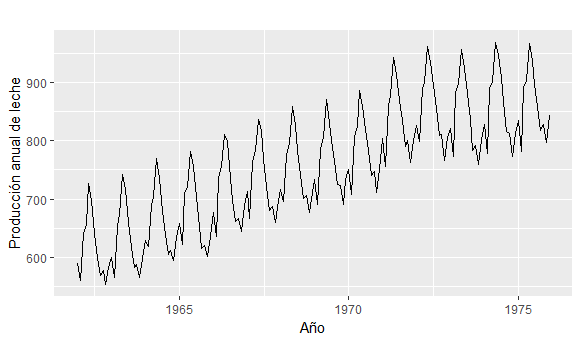
\includegraphics[width=.8\linewidth]{Images/Conceptos/leche.png}
  \caption{Estructura aditiva}
  \label{fig:sfig1}
\end{subfigure}
\begin{subfigure}{.5\textwidth}
  \centering
  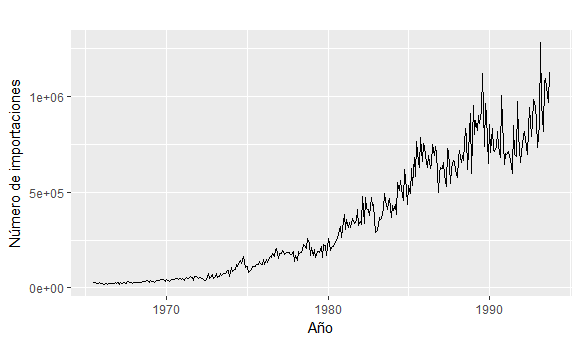
\includegraphics[width=.8\linewidth]{Images/Conceptos/importaciones.png}
  \caption{Estructura multiplicativa}
  \label{fig:sfig2}
\end{subfigure}
\caption{Comparación entre un modelo aditivo y multiplicativo}
\label{ad_mult}
\end{figure}

En la Figura \ref{ad_mult} se muestran ejemplos de ambos modelos. Identificar y entender el mecanismo que genera la serie temporal nos permitirá realizar predicciones fiables, además de ser capaces de entender mejor el proceso que genera los datos. Esto lo vamos a conseguir con la descomposición de la serie en subseries de acuerdo a las distintas componentes. Gracias a esta descomposición vamos a poder estudiar la evolución individual de cada componente, lo que nos permitirá identificar posibles patrones a fin de reproducir el comportamiento de la serie.

\subsection{Estimación de la tendencia}

Normalmente la tendencia es una de las componentes que más interesa estimar, ya que mediante técnicas sencillas podemos conocer la evolución a largo plazo de la serie. Existen varias técnicas para la extracción de la tendencia, el uso de unas u otras dependerá de la estructura y de la extensión de la serie que estemos estudiando.

En ocasiones la tendencia sigue un comportamiento fácilmente modelizable por una función $h(t)$ dependiente del tiempo $t$. La estimación de $h(t)$ se suele realizar por el método de los mínimos cuadrados. La estimación de los parámetros no va a suponer ningún problema gracias a la potencia computacional disponible hoy en día pero si lo supondrá la elección del modelo.

Algunas veces es sencillo identificar visualmente la función a usar para aproximar la tendencia ya que esta puede mostrar una evolución muy marcada (lineal, exponencial…). En caso contrario se puede probar a ajustar distintas funciones a fin de ver cuál de ellas se ajusta mejor. La elección de la función óptima se basa en indicadores estadísticos como el $R^2$ o la significatividad de los parámetros, aunque muchas veces basta con observar la serie temporal para decidirse por una u otra.

Algunas de las funciones más utilizadas para la estimación de la tendencia son:
\begin{description}
  \item[$\bullet$ Función lineal:]
      \begin{equation}
        h(t) = \alpha_0 + \alpha_1 t \quad con \quad \alpha_0, \alpha_1 \in \mathbb{R}
      \end{equation}
  \item[$\bullet$ Función cuadrática:]
      \begin{equation}
        h(t) = \alpha_0 + \alpha_1 t + \alpha_2 t^2 \quad con \quad \alpha_0, \alpha_1, \alpha_2 \in \mathbb{R}
      \end{equation}
  \item[$\bullet$ Función exponencial:]
      \begin{equation}
        h(t) = e^{\alpha_0 + \alpha_1 t} \quad con \quad \alpha_0, \alpha_1 \in \mathbb{R}
      \end{equation}
  \item[$\bullet$ Función logística:]
      \begin{equation}
        h(t) = \frac{e^{\alpha_0 + \alpha_1 t}}{1 + e^{\alpha_0 + \alpha_1 t}} \quad con \quad \alpha_0, \alpha_1 \in \mathbb{R}
      \end{equation}
\end{description}

En algunas ocasiones la serie temporal a estudiar no muestra un mismo comportamiento continuo a largo plazo por lo que ajustar este tipo de funciones supondría una gran pérdida de información. En este caso nos sería de gran utilidad ajustar un modelo que tuviese en cuenta intervalos más cortos de tiempo, facilitándonos así la visualización de la tendencia. El método de la media móvil se ajusta a esta problemática.

\subsubsection{Método de la media móvil}

Este método nos permite obtener una visualización rápida de la tendencia de la serie ya que trabaja con medias. Lo que hace es calcular medias de acuerdo a intervalos de longitud $p$, estos intervalos se van actualizando, eliminando la primera observación y añadiendo una nueva. Para calcular una media de orden $p$ sobre la serie $Y_t$ se recurre a lo siguiente:
\begin{equation}
    Y'_{t} = \frac{1}{p}\left(Y_{t-\left(\frac{p-1}{2}\right)}+...+Y_{t-1}+Y_t+Y_{t+1}+...+Y_{t+\left(\frac{p-1}{2}\right)}\right)
\end{equation}

Este método consigue eliminar el ruido y las fluctuaciones mediante los promedios, dejando a la vista la tendencia de la serie. En ocasiones hay que fijar $p$ de acuerdo a la estructura temporal de la serie para evitar extraer conclusiones erróneas sobre la tendencia.  Debido a la propia naturaleza del método incurrimos en una pérdida de $p$ observaciones.

\subsection{Estimación del ciclo}
La componente correspondiente al ciclo suele ser la más difícil de detectar y estimar, ya que aunque presenta variaciones más o menos recurrentes en el tiempo suelen ser resultado de la combinación de efectos muy variados con periodos diferentes. Debido a que muchas veces no es posible separar la tendencia del ciclo, estas dos componentes se estiman conjuntamente mediante las técnicas aplicadas a la estimación de la tendencia.

\subsection{Estimación de la estacionalidad}
Al igual que con la tendencia, existen varias aproximaciones a la hora de estimar la componente estacional. Debido a su naturaleza ondulatoria en ocasiones es posible aproximar esta componente a través de una función $g(t)$ periódica de periodo $s$:
\begin{equation}
    g(t) = g(t + s) = g(t + 2s)
\end{equation}

El periodo $s$ se corresponde al patrón de estacionalidad de la serie ($s = 4$ para datos trimestrales, $s = 12$ para datos mensuales…). Este tipo de funciones suelen estar formadas por una combinación de funciones armónicas. Estas técnicas suelen ajustarse  correctamente a estacionalidades con fluctuaciones complejas.

Otra forma de aproximar $g(t)$ es mediante variables \textit{dummy}. Estas variables recogen las variaciones debidas a la periodicidad estacional, de esta forma podemos expresar $g(t)$ como:
\begin{equation}
    g(t) = \sum_{i=1}^{S}(\lambda_{i} d_{it})
\end{equation}

\noindent donde $d_{it}$ son variables \textit{dummys} que toman el valor $1$ si el dato pertenece a ese periodo estacional y $0$ en caso contrario. El coeficiente $\lambda_{i}$ indica la variación correspondiente al periodo estacional $i$. Para estimar este factor estacional, si la estacionalidad es estable en el tiempo, basta con realizar la media de las observaciones correspondientes a cada periodo, en caso contrario no conviene resumir las distintas medias de cada periodo en un solo factor por que no describirá correctamente el comportamiento variable de la estacionalidad. En este último caso convendría ajustar alguna función matemática más compleja a esta componente.

\subsection{Estimación de la componente irregular}
El análisis de los residuos nos puede ser de gran utilidad a la hora de ver si hemos conseguido extraer correctamente todas las componentes. Sin los residuos (o componente irregular) no parecen mostrar ningún patrón, significa que hemos sido capaces de extraer todas las causas deterministas que componían la serie. Es posible obtener la componente irregular de la siguiente manera:
\begin{equation}
    Y_t - Y'_t - S_t = a_t
\end{equation}
\begin{equation}
    \frac{Y_t}{Y'_t \times S_t} = a_t
\end{equation}

En la Figura \ref{decomp} se muestra un ejemplo de descomposición de una serie temporal.
\begin{figure} [t]
\begin{subfigure}{.5\textwidth}
  \centering
  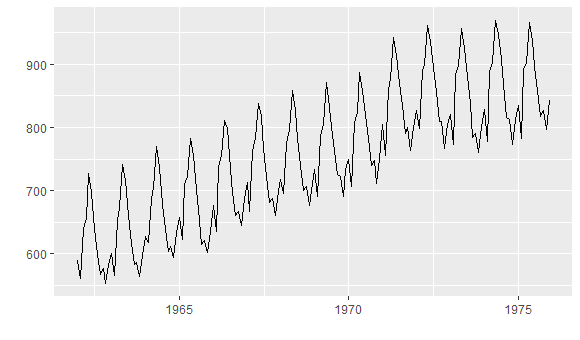
\includegraphics[width=.8\linewidth]{Images/Conceptos/serie.png}
  \caption{Serie original}
  \label{fig:sfig1}
\end{subfigure}
\begin{subfigure}{.5\textwidth}
  \centering
  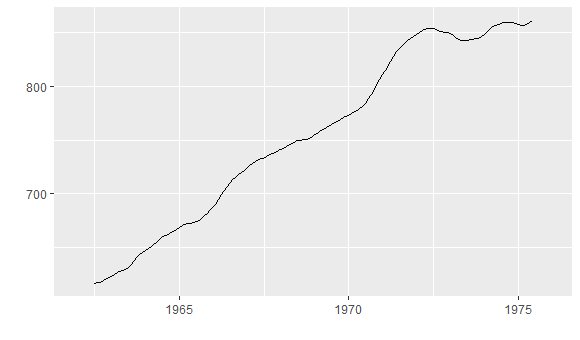
\includegraphics[width=.8\linewidth]{Images/Conceptos/tend.png}
  \caption{Tendencia}
  \label{fig:sfig2}
\end{subfigure}
\begin{subfigure}{.5\textwidth}
  \centering
  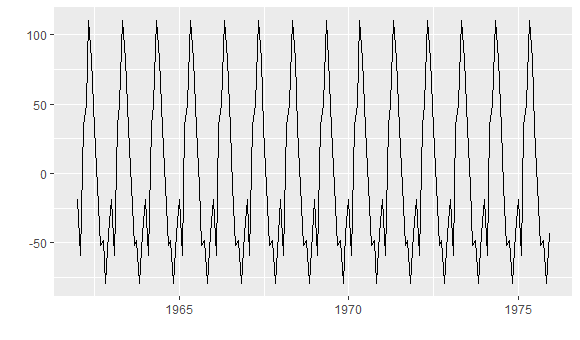
\includegraphics[width=.8\linewidth]{Images/Conceptos/season.png}
  \caption{Estacionalidad}
  \label{fig:sfig1}
\end{subfigure}
\begin{subfigure}{.5\textwidth}
  \centering
  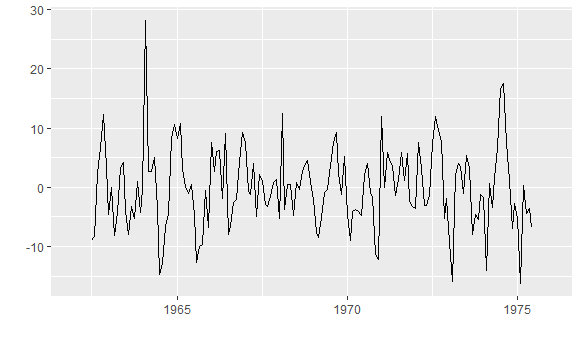
\includegraphics[width=.8\linewidth]{Images/Conceptos/random.png}
  \caption{Irregular}
  \label{fig:sfig2}
\end{subfigure}
\caption{Descomposición de la serie correspondiente a la producción de leche anual (Fuente:~\protect\citeNP{datamarket})}
\label{decomp}
\end{figure}


\subsection{Técnicas de suavizado}

Este tipo de técnicas nos permiten reducir o eliminar la aleatoriedad de la serie temporal permitiendo así una observación más nítida de sus componentes. Además nos ayudan a  predecir a corto plazo sin la necesidad de recurrir a modelos matemáticos complejos. Aunque este tipo de técnicas se pueden usar para cualquier tipo de serie temporal, suelen aplicarse más a aquellas que presentan una estructura inestable, con unas componentes menos marcadas o inexistentes debido a su naturaleza adaptativa a nivel local.

Uno de los suavizados más aplicados debido a su sencillez es el de medias móviles, ya explicado en apartados anteriores. Otros suavizados más complejos como el de \textit{splines} o \textit{kernel} (Anexo I) ofrecen también muy buenos resultados, aunque obviamente son mucho más costosos computacionalmente.

\subsubsection{Suavizado exponencial}
El suavizado exponencial es una media móvil ponderada en la que los valores más cercanos en el tiempo se ponderan más que los más alejados, a diferencia del suavizado de media móvil donde todos los valores influyen de igual manera.

El cálculo de la serie alisada se realiza de la siguiente manera:
\begin{equation}
   Y'_{t} = \alpha Y_{t} + (1 - \alpha)\thinspace Y_{t-1} + (1 - \alpha)^2 \thinspace Y_{t-2} + ... = \alpha \sum_{i=0}^{\infty} (1 - \alpha)^i \thinspace Y_{t-i} \quad \text{con} \quad 0 < \alpha < 1
\end{equation}

Como se puede apreciar, la serie alisada en el tiempo $t$ es resultado de la suma ponderada de todos los valores anteriores. Esta ponderación supone que los valores más recientes tienen una mayor influencia y esta influencia se va dispersando con el tiempo. Al parámetro $\alpha$ se le conoce como el factor de suavización y de él depende la importancia que se le da a los valores pasados y recientes. Este factor suele ser fijado por el investigador y dependerá principalmente de la estructura y evolución de la serie.

Se puede apreciar que para calcular cada nuevo valor alisado de la serie es necesario realizar los cálculos sobre todos los valores anteriores.  Para solventar este problema se suele recurrir a una expresión resultado de la aplicación de transformaciones matemáticas a la expresión (19) que da como resultado las siguientes fórmulas correspondientes al valor alisado y a la predicción de la serie, respectivamente:
\begin{equation}
   Y'_{t} = \alpha Y_{t} + (1 - \alpha)\thinspace Y'_{t-1}
\end{equation}
\begin{equation}
   \widehat{Y}_{t+1} = \alpha Y_{t} + (1 - \alpha)\thinspace \widehat{Y}_{t}
\end{equation}

Sabiendo esto podemos apreciar que:
\begin{equation}
   Y'_{2} = \alpha Y_{2} + (1 - \alpha)\thinspace Y'_{1}
\end{equation}

Por lo que el valor asignado a $Y'_{1}$ va a jugar un papel fundamental en el alisado de la serie. Existen varias posibilidades a elegir para fijar este valor (que sea igual a $Y_{1}$ o utilizar la media de la serie son algunas de ellas) que dependerán de la estructura y características propias de la serie.

Sabiendo esto, podemos apreciar mejor la importancia del factor de suavizado. Un $\alpha$ cercano a 0 significa que la parte alisada se tendrá más en cuenta y esto como consecuencia generará una suavización sin fluctuaciones. Un $\alpha$ cercano a 1 dará más peso a los valores más recientes de la serie generando así una suavización que tiene más en cuenta las fluctuaciones.

El suavizado aquí explicado es el simple y sirve de base para otros más complejos con una estructura también exponencial, capaces de adaptarse a tendencia y patrones estacionales mucho más complicados. En la Figura \ref{suav} se muestra un ejemplo de aplicación de estos suavizados.
\begin{figure} [t]
\begin{subfigure}{.5\textwidth}
  \centering
  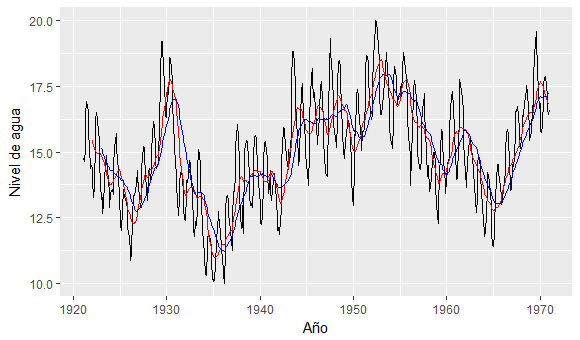
\includegraphics[width=.8\linewidth]{Images/Conceptos/ma.png}
  \caption{Medias móviles}
  \label{fig:sfig1}
\end{subfigure}
\begin{subfigure}{.5\textwidth}
  \centering
  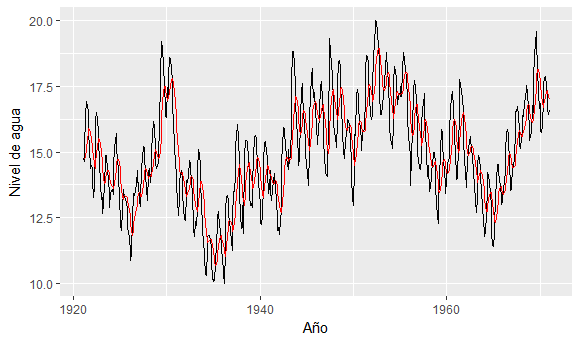
\includegraphics[width=.8\linewidth]{Images/Conceptos/exp.png}
  \caption{Exponencial simple}
  \label{fig:sfig2}
\end{subfigure}
\begin{subfigure}{.5\textwidth}
  \centering
  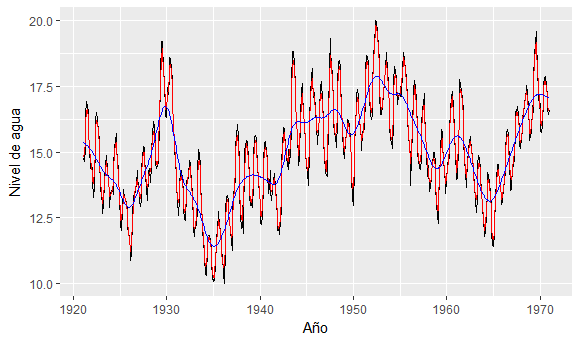
\includegraphics[width=.8\linewidth]{Images/Conceptos/ker.png}
  \caption{Kernel}
  \label{fig:sfig1}
\end{subfigure}
\begin{subfigure}{.5\textwidth}
  \centering
  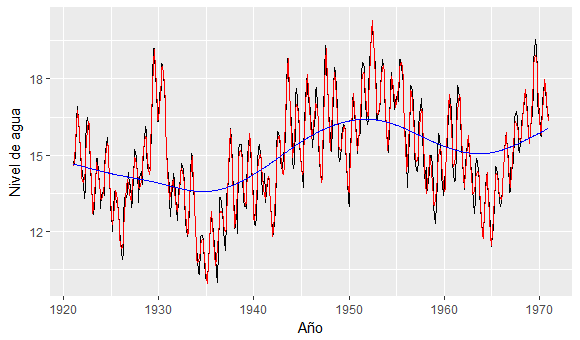
\includegraphics[width=.8\linewidth]{Images/Conceptos/spln.png}
  \caption{Spline}
  \label{fig:sfig2}
\end{subfigure}
\caption{Suavizado de la serie correspondiente al nivel mensual de agua del lago Erie (Fuente:~\protect\citeNP{datamarket})}
\label{suav}
\end{figure}


%%%%%%%%%%%%%%%%%%%%%%%%%%%%%%%%%%%%%%%%%%%%%%%%%%%%%%%%%%%%%%%%%%%%%%%%%%%%%%%%%%%%%%%%%%%%%%%%%%%%%%%%%%%%%%%%%%%%%%%%%%%%%%%%%%%%%%%%%%%%%%%%
%%%%%%%%%%%%%%%%%%%%%%%%%%%%%%%%%%%%%%%%%%%%%%%%%%%%%%%%%%%%%%%%%%%%%%%%%%%%%%%%%%%%%%%%%%%%%%%%%%%%%%%%%%%%%%%%%%%%%%%%%%%%%%%%%%%%%%%%%%%%%%%%


\section{Metodología Box-Jenkins}
La metodología Box-Jenkins fue desarrollada por George E. P. Box y Gwilym Jenkins en 1976 y se sustenta en los modelos ARIMA \cite{BoxJenkins2008}. Supone que la serie temporal es una realización de un proceso estocástico determinado y modelizable. Esta metodología busca encontrar un modelo que se ajuste a los datos y que nos permita realizar predicciones fiables a corto y medio plazo.

\subsection{Modelos ARIMA}
Para comprender este modelo vamos a realizar un pequeño recorrido por los distintos modelos que le componen.

\subsubsection{Procesos autorregresivos}
Algunas series temporales están muy influenciadas por sus valores pasados, en estos casos se ajusta un tipo de modelo autorregresivo en el que el valor presente de la variable depende de los valores pasados más una pequeña innovación contemporánea (parte aleatoria). Este modelo se conoce como autorregresivo y se suele denotar por las siglas AR. Si la variable se ve influenciada por sus valores pasados hasta el retardo $t-p$ hablamos de un modelo autorregresivo de orden $p$ o AR($p$). Sabiendo esto, podemos definir el modelo de la siguiente manera:
\begin{equation}
    Y_{t}=\phi_{1} Y_{t-1} + \phi_{2} Y_{t-2} + \phi_{3} Y_{t-3}+...+\phi_{p} Y_{t-p}+a_{t}
\end{equation}

\noindent con $\phi_i$ parámetros a estimar y $a_{t}$ ruido blanco.

Para estudiar la estacionariedad vamos a expresar el modelo mediante su operador de retardos:
\begin{equation}
    (1-\phi_{1}L-\phi_{2}L^{2}-...-\phi_{p}L^{p})Y_{t} = a_{t}
\end{equation}

\begin{equation}
    \phi_{p}(L)Y_{t} = a_{t}
\end{equation}

\noindent donde $\phi_{p}(L)$ se conoce como polinomio autorregresivo, siendo $(\phi_{1};\phi_{2};...;\phi_{p})$ su vector de parámetros. Este polinomio va a tener generalmente $p$ raíces diferentes por lo que se puede expresar como:
\begin{equation}
    \phi_{p} = \prod_{i=1}^{p}(1-L_{i}^{-1}L)
\end{equation}

Está demostrado que este proceso será estacionario si y solo si el módulo de las raíces de su polinomio autorregresivo está fuera del círculo unidad:
\begin{equation}
    \mid L_{i}^{-1}\mid < 1 \quad \forall{i}
\end{equation}

Además para poder garantizar completamente la estacionariedad de un proceso autorregresivo, éste debe depender  únicamente de su pasado y no de su futuro, lo cual se cumple en la mayor parte de series temporales y además debe ser invertible, es decir, debe cumplirse que:
\begin{equation}
    \sum_{i=1}^{p} \phi_{i}^{2} < \infty
\end{equation}

La función de autocorrelación se caracteriza por aproximarse a cero conforme $k \rightarrow \infty$, pudiendo ser este decrecimiento oscilante.

\subsubsection{Procesos de medias móviles}
En ocasiones se dan casos en los que para una serie temporal determinada, un modelo en el que el valor actual depende de las innovaciones contemporáneas y pasadas hasta el retardo $t-q$ se ajusta correctamente. Los modelos sustentados en estos principios se conocen como modelos de medias móviles de orden $q$ o MA($q$), se definen de la siguiente forma:
\begin{equation}
    Y_{t} =  a_{t}-\theta_{1}a_{t-1}-\theta_{2}a_{t-2}-...-\theta_{q}a_{t-q}
\end{equation}

\noindent con $\theta_i$ parámetros a estimar y $a_{t-i}$ ruido blanco.

Si procedemos como antes, tenemos que este proceso se puede representar mediante el operador de retardos:
\begin{equation}
    Y_{t} = \theta_{q}(L)a_{t}
\end{equation}

\noindent donde el polinomio de medias móviles se puede expresar a través de sus $q$ raíces:
\begin{equation}
    \theta_{q}(L) =  \prod_{i=1}^{q}(1-L_{i}^{-1}L)
\end{equation}

No es necesario imponer ninguna restricción sobre los parámetros $\theta_{1}, \theta_{2},...,\theta_{q}$ para garantizar la estacionariedad, sin embargo se necesita que el módulo de las raíces del polinomio de medias móviles esté fuera del círculo unidad para garantizar la invertibilidad:
\begin{equation}
\mid L_{i}^{-1}\mid < 1 \quad \forall{i}
\end{equation}

En este caso la función de autocorrelación se caracteriza por sufrir un corte abrupto a partir del retardo $q$.

\subsubsection{Procesos autorregresivos de medias móviles}
Este modelo determina el valor de $Y_{t}$ a partir de su pasado hasta el retardo $p$, de su innovación contemporánea y de las pasadas hasta el retado $q$. Se denota como ARMA($p$,$q$) y su expresión es la siguiente:
\begin{equation}
    Y_{t} = a_{t} + \sum_{i=1}^{p} \phi_{i} Y_{t-i} + \sum_{i=1}^{q} (-\theta_{i}) a_{t-i}
\end{equation}

Al tratar con ambos procesos a la vez en términos del operador de retardos tenemos lo siguiente:
\begin{equation}
    \phi_{p}(L)Y_{t} = \theta_{q}(L)a_{t}
\end{equation}

La estacionariedad del proceso dependerá de las condiciones de la parte autorregresiva, es decir, será estacionario siempre que el módulo de las raíces del polinomio autorregresivo esté fuera del círculo unidad, y la invertibilidad de la parte de medias móviles, o lo que es lo mismo, el módulo de las raíces del polinomio de medias móviles debe estar fuera del círculo unidad.

La función de autocovarianzas se caracteriza por ser infinita y la de autocorrelación por decrecer rápidamente hacia cero a medida que aumenta $k$.

\subsubsection{Procesos autorregresivos integrados de medias móviles}
Hemos visto que un proceso ARMA es estacionario si su parte autorregresiva lo es. La no estacionariedad del modelo se puede presentar entonces de dos formas distintas:
\begin{equation}
\mid L_{i}^{-1}\mid > 1 \quad \forall{i}
\end{equation}
\begin{equation}
\mid L_{i}^{-1}\mid = 1 \quad \forall{i}
\end{equation}

\noindent siendo $L_{i}$ las raíces del polinomio autorregresivo. En economía, que es dónde usualmente se utilizan este tipo de modelos, lo común es encontrarse con el segundo caso (raíz unitaria) en el que cual la serie se comporta más o menos igual a lo largo del tiempo variando únicamente de nivel. Para solucionar esto se recurren a los modelos autorregresivos integrados de medias móviles o ARIMA. Para ver cómo funcionan comencemos factorizando la parte autorregresiva del modelo general:
\begin{equation}
\phi_{p}(L)Y_{t} = (1-L_{1}^{-1}L)\cdot(1-L_{2}^{-1}L)\cdot...\cdot(1-L_{p}^{-1}L)
\end{equation}

Supongamos que tenemos $d$ raíces unitarias en esta parte autorregresiva, en ese caso podremos agrupar de la siguiente forma:
\begin{equation}
\phi_{p}(L)Y_{t} = \gamma_{p-d}(L)\cdot(1-L)^{d}
\end{equation}

Hemos agrupado las $d$ raíces unitarias en el término $(1-L)^{d}$ por lo que si ahora sustituimos en el modelo general tenemos que:
\begin{equation}
\gamma_{p-d}(L)\cdot(1-L)^{d}\cdot Y_{t}=\theta_{q}(L)a_{t}
\end{equation}
\begin{equation}
\gamma_{p-d}(L)\cdot\Delta^{d}Y_{t}=\theta_{q}(L)a_{t}
\end{equation}

Aquí $\gamma_{p-d}(L)$ es estacionario ya que no incluye a las raíces unitarias dado que las hemos conseguido eliminar diferenciando $Y_{t}$ $d$ veces. Por lo tanto ahora tenemos que el proceso que define a $\Delta^{d}Y_{t}$ es estacionario. Conociendo esto podemos afirmar que un modelo ARIMA no es más que un modelo ARMA diferenciado $d$ veces por lo que está compuesto de los parámetros $p$, $d$ y $q$, ARIMA($p, d, q$).

Como se puede apreciar el modelo ARIMA aúna las principales características de otros modelos. El objetivo de la metodología Box-Jenkins va a ser elegir los valores óptimos de los parámetros que definen al ARIMA para asegurarnos un ajuste óptimo de nuestros datos.

\subsection{Etapas}
En un principio la metodología Box-Jenkins estaba compuesta por tres etapas pero con el paso del tiempo han sido varios los autores que han defendido añadir alguna más \cite{etapas}. Nosotros consideraremos las siguientes etapas:
\begin{itemize*}
    \item[$\bullet$]Preparación de los datos
    \item[$\bullet$]Identificación y selección del modelo
    \item[$\bullet$]Estimación de los parámetros
    \item[$\bullet$]Validación del modelo
    \item[$\bullet$]Predicción
\end{itemize*}

\subsubsection{Preparación de los datos}
Como ya hemos visto, para que una serie sea estacionaria es necesario que no tenga tendencia y que la varianza sea constante. En la mayor parte de casos es posible observar esto mediante el estudio gráfico de los datos. Si nuestra serie muestra una evolución a largo plazo con pendiente, o la varianza parece evolucionar en el tiempo, es posible que nos encontremos ante una caso de no estacionariedad y necesitaremos tratar nuestra serie a fin de poder aplicar esta metodología.

En otras ocasiones, bien porque la gráfica no nos aporta mucha información o bien porque queremos asegurarnos estadísticamente de la estacionariedad de la serie, se recurre a distintos test estadísticos capaces de contrastar la estacionariedad de la serie estudiada. Uno de los más conocidos es la prueba de la raíz unitaria de Dickey Fuller.

En el caso de trabajar bajo no estacionariedad en tendencia se recomienda diferenciar la serie hasta conseguir eliminarla. Es aquí donde se define el valor del parámetro $d$ del ARIMA.

Si estamos tratando con una serie no estacionaria en varianza se suele recomendar aplicar alguna transformación a los datos que estabilice la varianza. Suele funcionar muy bien aplicar logaritmos a la serie aunque en ocasiones también se suele aplicar la transformación Box-Cox ya que además consigue aproximar la distribución de $Y_t$ a una normal:
\begin{equation}
Z(\lambda) =
\begin{cases}
\frac{y^\lambda - 1}{\lambda} & \text{si } \lambda \neq 0 \\
\log(y) & \text{si } \lambda = 0
\end{cases}
\end{equation}

\subsubsection{Identificación y selección del modelo}
Una vez preparada la serie debemos identificar el modelo a ajustar. En esta fase lo que principalmente se busca es elegir los valores óptimos de $p$ y $q$. Observando la FAC y FACP podemos estudiar la evolución de la autocorrelación de la serie, pudiendo así identificarla con alguna estructura típica de los distintos modelos estudiados.

En apartado anteriores hemos visto que por definición la FAC de un proceso autorregresivo se aproxima a cero conforme $k \rightarrow \infty$ y que la FAC de un proceso de medias móviles sufre un corte abrupto a partir del retardo $q$. A partir de este tipo de características es posible construir la Tabla \ref{identificacion}. Este tipo de tablas nos aportan información valiosa para una selección óptima del modelo.

\begin{table}[]
\centering
\label{my-label}
\begin{tabular}{|l|c|c|}
\hline
\multicolumn{1}{|c|}{} & FAC                            & FACP                           \\ \hline
AR($p$)                  & Decrece sin anularse           & Se anula para $j \textgreater p$ \\ \hline
MA($q$)                  & Se anula para $j \textgreater q$ & Decrece sin anularse           \\ \hline
ARMA($p,q$)              & Decrece sin anularse           & Decrece sin anularse           \\ \hline
\end{tabular}
\caption{Identificación de los distintos modelos}
\label{identificacion}
\end{table}

En la Figura \ref{comp_acf_pacf} se muestran las FAC teóricas para algunos modelos. Este tipo de identificación tiene un pequeño componente subjetivo debido a la propia interpretación de los correlogramas por lo que la experiencia del investigador juega un papel fundamental en la selección del modelo.

\begin{figure} [t]
\begin{subfigure}{.5\textwidth}
  \centering
  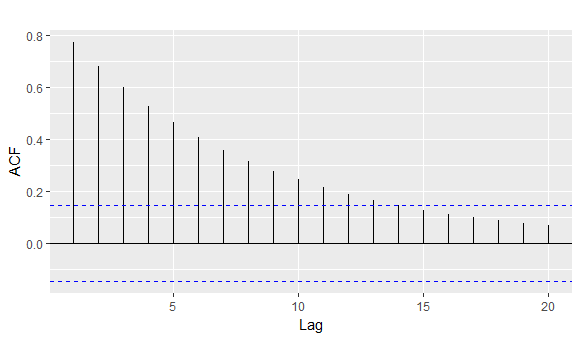
\includegraphics[width=.8\linewidth]{Images/Conceptos/ar_teorico.png}
  \caption{FAC de un proceso autorregresivo}
  \label{fig:sfig1}
\end{subfigure}
\begin{subfigure}{.5\textwidth}
  \centering
  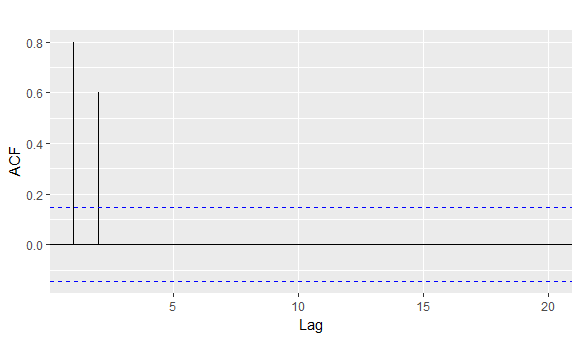
\includegraphics[width=.8\linewidth]{Images/Conceptos/ma_teorico.png}
  \caption{FAC de un proceso de medias móviles}
  \label{fig:sfig2}
\end{subfigure}
\caption{Correlogramas teóricos}
\label{comp_acf_pacf}
\end{figure}

\subsubsection{Estimación de los parámetros}
Una vez transformada la serie y seleccionado el modelo ARIMA a ajustar, es necesario estimar los parámetros. Existen multitud de métodos numéricos aplicados al cálculo de estos parámetros aunque quizás los más utilizados sean el método de máxima verosimilitud y el de mínimos cuadrados no lineales.

En ocasiones debido a problemas de no linealidad la maximización de la función de verosimilitud se realiza a través de métodos numéricos, es por esto por lo que el valor inicial de los parámetros es clave para garantizar una buena convergencia hacia el máximo. Existen varios métodos orientados al cálculo de estos valores (método de Yule-Walker, algoritmo de Burg, algoritmo de Hannan-Rissanen, etc…).

La potencia computacional necesaria para la estimación es tal que se resulta enormemente complicado realizar el cálculo manualmente. Generalmente no resulta necesario preocuparse por la estimación de los parámetros ya que se suele llevar a cabo automáticamente por rutinas ya implementadas en software estadístico especializado.

\subsubsection{Validación del modelo}
Una vez hemos elegido el modelo a ajustar y estimados sus parámetros debemmos comprobar si efectivamente se está realizando un buen ajuste, es decir, si nuestro modelo es válido.

Si el modelo ajustado explica correctamente nuestros datos no debemos esperarnos ningún tipo de patrón en los residuos, es decir, se deben comportar como ruido blanco. Una forma de comprobar esto es mediante la FAC y FACP de los residuos. Si esperamos que los residuos sean ruido no deberíamos observar correlaciones entre ellos, lo que significa que ninguna autocorrelación debería ser significativamente distinta de cero. Para comprobar esto definimos unas bandas de confianza al 95$\%$ para los correlogramas:
\begin{equation}
    \left[-\frac{1.96}{\sqrt{T}}, \frac{1.96}{\sqrt{T}}\right]
\end{equation}

\noindent siendo $T$ el número de valores de nuestra serie temporal.

Otra forma de estudiar los residuos es mediante la aplicación de test de contraste de hipótesis, los dos más usados son el de Box-Pierce y una variante de este conocida como Ljung-Box. Con estos estadísticos somos capaces de contrastar si las correlaciones entre los residuos son iguales a cero o no. Aunque ambos estadísticos funcionan bien en muestras grandes parece que el de Ljung-Box se comporta mejor en muestras pequeñas, es por esto lo que se ha extendido la utilización de este último:
\begin{equation}
   LB = T(T + 2) \sum_{k = 1}^{m} \frac{\hat{\rho}^2_{k}}{T-k}
\end{equation}

\noindent donde $\hat{\rho}_{k}$ es el coeficiente de autocorrelación de los residuos estimados hasta el retardo $k$ y $m$ el número de retardos sobre los que estamos trabajando. Este estadístico se distribuye bajo una Chi-Cuadrado con $m – p – q$ grados de libertad.

Además de los residuos conviene también tener en cuenta otros aspectos del modelo como la significatividad de los coeficientes o el poder predictivo. Al fin y al cabo es el investigador el que considera si el modelo es el correcto para sus datos.
	
Si el modelo no es válido se selecciona otro, se estiman los nuevos coeficientes y se vuelve a validar. El proceso se repite hasta que se encuentre un modelo que satisfaga las necesidades del investigador.

\subsubsection{Predicciones}
Una vez seleccionado y validado el modelo debemos predecir. Supongamos que hemos ajustado un ARMA($p, q$) a nuestra serie y queremos predecir $Y_{t + h}$, para ello debemos calcular:
\begin{equation}
    \widehat{Y}_{t + h} = a_{t + h} + \sum_{i=1}^{p} \widehat{\phi}_{i} \widehat{Y}_{t+h-i} + \sum_{i=1}^{q} (-\widehat{\theta}_{i}) a_{t+h-i}
\end{equation}

\noindent donde $a_{t + h} = 0$, $\widehat{Y}_{t+h-i}$ son las predicciones realizadas en tiempos anteriores y $a_{t+h-i}$ los residuales de esas predicciones. Se puede apreciar como para calcular la parte autorregresiva y medias móviles de la serie en el tiempo $t + h$ se ha necesitado realizar las predicciones para los tiempos $t+1,...,t+h-1$.

Es posible calcular los intervalos de confianza de estas predicciones, pero para ello tenemos que asegurarnos de que los residuos sean ruido, en caso contrario puede que los intervalos sean erróneos. Estos intervalos se amplían a medida que nos alejamos en las predicciones, llegando a converger en horizontes lejanos de la serie.


\newpage
\part{Estructura de los datos temporales en $\textsf{R}$}
\lhead [\thepage]{III. Estructura de los datos temporales en $\textsf{R}$}
\rhead [III. Estructura de los datos temporales en $\textsf{R}$]{\thepage}
\setcounter{section}{0}

\section{Introducción}
Las series temporales están constituidas por una sucesión de fechas o momentos temporales que conforman el índice y los valores de la variable en cada uno de estos momentos. El principal objeto usado en $\textsf{R}$ para almacenar datos es el $\verb!data.frame!$, ya que permite aunar variables de distintas clases en un mismo objeto fácilmente manipulable, sin embargo no es válido para las series temporales. En estos casos se necesita definir nuevos objetos capaces de almacenar datos temporales y que además permitan un amplio tratamiento a través de los distintos métodos implementados en $\textsf{R}$.

Son varias las librerías encargadas de definir objetos específicos para almacenar datos temporales. Todas ellas implementan los mismos métodos básicos pero orientados a su clase particular. En este apartado se hablará de aquellas indispensables para el correcto análisis estadístico de nuestras series.

En este apartado trabajaremos con la serie correspondiente al número de vehículos vendidos en Quebec durante los años comprendidos entre 1960 y 1968 \cite{datamarket}. El código utilizado se muestra en el Anexo II.

\section{Stats Package}
La librería $\verb!stats!$ es una de las que componen la base de $\textsf{R}$. Se encuentra ya instalada por defecto en el propio lenguaje y se carga automáticamente una vez le iniciamos. Una parte de esta librería está dedicada al tratamiento de series temporales \cite{stats}.

Por defecto en $\textsf{R}$ las series temporales se deben estructurar en un objeto de clase $\verb!ts!$. Para convertir nuestros datos temporales univariantes a este formato debemos utilizar el método $\verb!ts()!$:
\begin{Verbatim}[fontsize=\footnotesize]
    ts(data = NA, start = 1, end = numeric(), frequency = 1, ...)
\end{Verbatim}

A esta función se la asigna el vector que recoge las observaciones de nuestra variable ordenadas cronológicamente a través de $\verb!data!$, la fecha de inicio de la serie a través de $\verb!start!$ y la frecuencia en la que se han recogido las observaciones a través de $\verb!frequency!$. Aunque estos dos últimos argumentos no son obligatorios sí son recomendables para tener nuestra serie correctamente estructurada.

Se debe tener mucho cuidado con el formato de las fechas en $\textsf{R}$. Para convertir una cadena en fecha es necesario recurrir a la función $\verb!as.Date()!$ y tener precaución al especificar el formato de entrada de la cadena ($\verb!format!$). Este tipo de objeto está limitado a serie espaciadas regularmente (mensuales, cuatrimestrales, anuales…) por lo que necesitaremos otras librerías que dispongan de una estructuración más avanzada si queremos tratar con series más complejas temporalmente.

Para represenar gráficamente estos objetos se recurre a un método  derivado de $\verb!plot()!$ conocido como $\verb!plot.ts()!$(la sintaxis de los argumentos de ambos métodos es la misma). Para seleccionar un subconjunto de nuestra serie recurrimos a la función $\verb!window()!$:
\begin{Verbatim}[fontsize=\footnotesize]
    window(x, start = NULL, end = NULL)
\end{Verbatim}

En la Figura \ref{window} se muestra un ejemplo de selección de observaciones a través de $\verb!window()!$.
\begin{figure}
    \centering
    \centerline{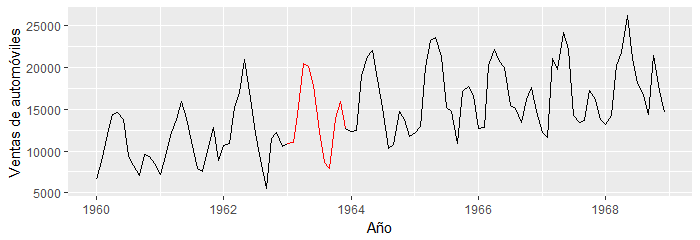
\includegraphics[scale = 0.7]{Images/Estructura/window.png}}
    \caption{Selección de las observaciones correspondientes a 1963 de la serie de ventas mensuales de automóviles en Quebec}
    \label{window}
\end{figure}

Es posible unir varias series temporales en un mismo objeto, para ello se suele recurrir al método $\verb!cbind()!$. La clase de este nuevo objeto pasa a ser $\verb!mts!$ que no es más que la clase $\verb!ts!$ extendida a series multivariantes.

Existen varios métodos más enfocados a realizar operaciones sencillas sobre series temporales que serán abordados en los apartados correspondientes a las librerías $\verb!zoo!$ y $\verb!xts!$ (aunque se aplican sobre objetos de clases distintas suelen presentar un comportamiento y una sintaxis similar).


\section{Zoo Package}
A diferencia de $\verb!stats!$, esta librería permite una estructuración de los datos más avanzada llegando incluso a poder almacenar series con intervalos de tiempo irregulares. La clase $\verb!zoo!$ combina el índice temporal y los datos en un mismo objeto facilitando así su tratamiento. La función encargada de estructurar los datos es $\verb!zoo()!$:
\begin{Verbatim}[fontsize=\footnotesize]
zoo(x = NULL, order.by = index(), frequency = NULL)
\end{Verbatim}

En este caso debemos introducir un vector con los valores de la variable ordenados cronológicamente y una frecuencia (igual que en $\verb!ts()!$) o un vector con las fechas ya generadas. Una función muy útil para generar una secuencia de fechas es $\verb!seq.Date()!$. Aunque en ocasiones es más sencillo generar la serie a partir de $\verb!ts()!$, suele ser necesario utilizar clases más extendidas como $\verb!zoo!$. El método $\verb!as.zoo()!$ se encarga de realizar la conversión entre estos objetos \cite{zoo}.

Es posible generar fechas mensuales y trimestrales a partir de las funciones $\verb!yearmon()!$ y $\verb!yearqtr()!$. El vector de fechas introducido como argumento a $\verb!zoo()!$ a través de $\verb!order.by!$ suele ser un objeto de clase $\verb!date!$, $\verb!yearmon!$ o $\verb!yearqtr!$ aunque existen otros más complejos capaces de almacenar el factor tiempo a través de minutos, horas, etc.

Es posible extraer el índice y las observaciones de nuestras variables a través de las funciones $\verb!index()!$ y $\verb!coredata()!$. Esto es muy útil para algunos métodos más restrictivos respecto a los argumentos que acepta. Una de las ventajas de esta clase de objetos es la posibilidad de seleccionar observaciones a través de la fecha. Si tenemos una serie mensual ($\verb!sales!$) comprendida entre los años 1960 y 1968 y queremos conocer los valores correspondientes al año 1963 basta con ejecutar la siguiente sentencia:
\begin{Verbatim}[fontsize=\footnotesize]
sales[seq.Date(from = as.Date("1963-01-01"), to = as.Date("1963-12-01"), by = "month")]
\end{Verbatim}

Para combinar varias series temporales en un mismo objeto basta con usar $\verb!merge.zoo()!$. En caso de que el intervalo temporal sea distinto este método completa los datos faltantes con $\verb!NAs!$, ofreciéndonos así como salida un objeto $\verb!zoo!$ totalmente operativo conformado por las series iniciales.

El tratamiento de los $\verb!NAs!$ suele ser un tema delicado en el que los investigadores no acaban de ponerse de acuerdo. Esta librería contiene varios métodos enfocados a esta problemática:
\begin{itemize*}
  \item[$\bullet$] \PVerb{na.aggregate()}: Permite remplazar los  $\verb!NAs!$ a través de datos basados en funciones como la media.
  \item[$\bullet$] \PVerb{na.approx()}: Sustituye los $\verb!NAs!$ a través de una interpolación lineal.
  \item[$\bullet$] \PVerb{na.spline()}: Recurre a la interpolación cúbica de splines para remplazar los $\verb!NAs!$.
  \item[$\bullet$] \PVerb{na.fill()}: Nos permite sustituir los $\verb!NAs!$ por los valores que queramos. Estos valores se introducen como vector a través del argumento $\verb!fill!$. También es posible la sustitución de los $\verb!NAs!$ a través de los valores adyacentes.
  \item[$\bullet$] \PVerb{na.locf()}:Sustituye los $\verb!NAs!$ por su valor más cercano en el tiempo. Es una implementación más directa del método anterior.
\end{itemize*}

Es posible retrasar la serie hacia delante o hacia atrás en el tiempo gracias al método $\verb!lag()!$:
\begin{Verbatim}[fontsize=\footnotesize]
lag(x, k = 1, na.pad = FALSE,...)
\end{Verbatim}

El objeto $\verb!zoo!$ se introduce al partir del argumento $\verb!x!$ y el rezago que deseamos aplicar a la serie a partir de $\verb!k!$. Es importante activar $\verb!na.pad!$ para no perder las fechas vinculadas al retardo $k$, ya que lógicamente con este retraso perderemos $k$ observaciones. Si $\verb!k!$ es positivo desplazamos la serie hacia delante y si es negativo hacia atrás.

Es posible utilizar $\verb!plot()!$ con objetos $\verb!zoo!$ para visualizar la evolución de la serie temporal. Al tratarse de la función $\verb!plot()!$ la sintaxis es similar a la que se suele usar normalmente para representar otros objetos más comunes en $\textsf{R}$. Esta librería contiene algunos métodos más completos para estos propósitos como puede ser $\verb!plot.zoo()!$ que facilita enormemente la representación de series temporales multivariantes.

Existen métodos que facilitan la lectura de datos. Lo más común es leer los datos desde un archivo $\verb!.csv!$ o $\verb!.txt!$ para almacenarlos en un $\verb!data.frame!$ y a partir de ahí realizar las transformaciones necesarias a fin de almacernarlos en un objeto $\verb!zoo!$. Los métodos $\verb!read.zoo()!$ y $\verb!read.csv.zoo()!$ nos ahorran este proceso y nos permiten pasar directamente de la lectura al objeto $\verb!zoo!$. En ocasiones es conveniente pasar a la función algún método a través del argumento $\verb!FUN!$ para tratar las fechas del archivo de origen .

En ocasiones nos puede interesar aplicar cierta función a nuestra serie de forma gradual, es decir, por grupos de observaciones. El método usado para este tipo de tareas es $\verb!rollapply()!$:
\begin{Verbatim}[fontsize=\footnotesize]
rollapply(data, width, FUN, align)
\end{Verbatim}

El argumento $\verb!data!$ recoge nuestro objeto $\verb!zoo!$ y $\verb!width!$ el número de observaciones sobre el que vamos a ir pasando la función recogida en $\verb!FUN!$. El argumento $\verb!align!$ nos permite decidir dónde queremos que empiece la ordenación cronológica del objeto $\verb!zoo!$ resultante. Por ejemplo, si tenemos:
\begin{Verbatim}[fontsize=\footnotesize]
rollapply(sales, 12, sum, align = "right")
\end{Verbatim}

Lo que realmente estamos haciendo es:
\begin{Verbatim}[fontsize=\footnotesize]
         sum(sales[1:12])
         sum(sales[2:13])
         sum(sales[3:14])
         ...
\end{Verbatim}

El resultado será un objeto $\verb!zoo!$ con una observación menos al final de la serie. El argumento $\verb!by!$ nos va a permitir aplicar la función elegida a cada intervalo de longitud $\verb!by!$ sin repetir observaciones.

Un método derivado de este último es $\verb!rollmean()!$. Gracias a él podemos suavizar nuestra serie a través de una media móvil de orden $k$. Para asegurarnos de que el cálculo se realiza únicamente con las observaciones pasadas debemos indicar que $\verb!align = "right"!$. Por ejemplo, para aplicar una media móvil de orden 12 que solo realice los cálculos con las observaciones de momentos ya transcurridos debemos escribir:
\begin{Verbatim}[fontsize=\footnotesize]
rollmean(x = sales, k = 12, align = "right")
\end{Verbatim}

Se puede apreciar fácilmente que es posible implementar $\verb!rollmean()!$ a través de $\verb!rollapply()!$. Para decidirnos por una u otra vamos a medir el tiempo de ejecución de cada una y para ello utilizaremos el método de la base de $\textsf{R}$ $\verb!system.time()!$. Este método toma como entrada una expresión a evaluar y nos devuelve tres valores:
\begin{itemize*}
  \item[$\bullet$] \textbf{User time}: Tiempo de ejecución llevado a cabo en la CPU.
  \item[$\bullet$] \textbf{System time}: Tiempo de ejecución llevado a cabo en el sistema operativo (lectura de datos, control de tiempos…)
  \item[$\bullet$] \textbf{Elapsed time}: Tiempo total transcurrido en la ejecución desde que se inició el proceso. Este tiempo es el que se utiliza para hacer el \textit{timing} del proceso.
\end{itemize*}

Para medir el tiempo de ejecución de cada método hemos generado una serie temporal con $10^5$ observaciones generadas a partir de una distribución normal con media 200 y desviación típica 20. A continuación se muestra el código empleado:
\begin{Verbatim}[fontsize=\footnotesize, numbers = left]
data <- zoo(rnorm(100000, 200, 20))
system.time(rollmean(x = data, k = 12, align = "right"))
system.time(rollapply(data = data, width = 12, FUN = mean, align = "right"))
\end{Verbatim}

El tiempo de ejecución en segundos llevado a cabo por $\verb!rollmean()!$ y $\verb!rollapply()!$ respectivamente es:
\begin{Verbatim}[fontsize=\footnotesize]
user  system elapsed
0.20    0.00    0.21

user  system elapsed
0.22    0.00    0.22
\end{Verbatim}

Como se puede apreciar estamos obteniendo tiempos similares. Para conseguir apreciar mejor la diferencia entre los métodos vamos a llevar a cabo una simulación. Ejecutaremos los dos métodos 100 veces para cantidades distintas de datos y después tomaremos la media de los tiempos para intentar eliminar el ruido inherente a la medición de los tiempos, los resultados se muestran en la Figura \ref{times_1}. Se puede ver como para números moderados de observaciones ambos se comportan parecido pero para números grandes $\verb!rollapply()!$ parece funcionar mejor que $\verb!rollmean()!$.

\begin{figure}
    \centering
    \centerline{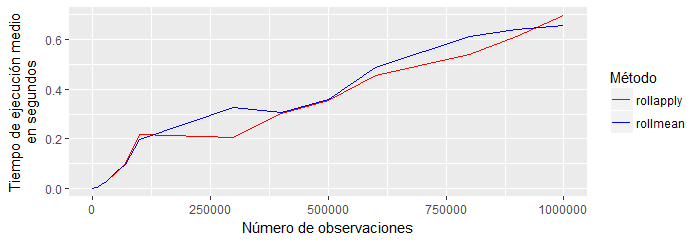
\includegraphics[scale = 0.7]{Images/Estructura/timing-roll.png}}
    \caption{Comparación de tiempos de ejecución para los métodos \PVerb{rollapply()} y \PVerb{rollmean()}}
    \label{times_1}
\end{figure}

\section{XTS Package}
Esta librería introduce una nueva clase de objetos conocida como $\verb!xts!$. Esta clase está basada en $\verb!zoo!$ pero tiene la gran peculiaridad de ser totalmente extensible a cualquier otra clase de datos temporales en $\textsf{R}$, es decir, da igual el formato en el que tengamos nuestros datos ya que siempre va a ser posible transformarlos a la clase $\verb!xts!$ \cite{xts}.

Al igual que con $\verb!zoo!$, para crear un objeto $\verb!xts!$ se debe usar el método $\verb!xts()!$ que se define de la siguiente manera:
\begin{Verbatim}[fontsize=\footnotesize]
xts(x = NULL, order.by = index(x), frequency = NULL, unique = TRUE,…)
\end{Verbatim}

Lo realmente interesante de este paquete es su capacidad de aunar cualquier estructura temporal. Existen muchos objetos capaces de almacenar nuestros datos ($\verb!ts!$, $\verb!zoo!$, $\verb!timeSeries!$, $\verb!matrix!$, $\verb!data.frame!$…) y todos ellos pueden ser convertidos a $\verb!xts!$ a través del método $\verb!as.xts()!$:
\begin{Verbatim}[fontsize=\footnotesize]
as.xts(x,...)
\end{Verbatim}

En un principio puede parecer inútil almacenar una serie temporal en un objeto $\verb!matrix!$ o $\verb!data.frame!$ pero es muy útil si se quiere trabajar con series temporales multivariantes.

Esta clase de objeto está equipada con un sistema de selección de observaciones realmente intuitivo y útil. A continuación mostraremos un ejemplo de esta característica aplicada a una nuestra serie mensual $\verb!xts.sales!$:
\begin{Verbatim}[fontsize=\footnotesize, numbers = left]
# diciembre de 1963
xts.sales["1963-12"]
# el año completo de 1963
xts.sales["1963"]
# todas las observaciones hasta julio de 1963
xts.sales["/1963-7"]
# todas las observaciones a partir de julio de 1963
xts.sales["1963-7/"]
# observaciones comprendidas entre julio de 1962 y de 1963
xts.sales["1962-7/1963-7"]
\end{Verbatim}

Al ser $\verb!xts!$ una extensión de $\verb!zoo!$ todos los métodos de este último se pueden aplicar al primero sin necesidad de modificar las entradas de los argumentos. Algunos de estos métodos como $\verb!index()!$ o $\verb!merge()!$ detectan la clase del objeto y se adaptan a él ejecutándose automáticamente como $\verb!index.xts()!$ y $\verb!merge.xts()!$.

Esta librería incluye también métodos bastante más avanzados para el tratamiento de formatos y estructuras, razón por la cual los analistas más expertos se suelen decantar por ella.

Existen también un conjunto de métodos para objetos $\verb!xts!$ encargados de iterar a través de series y aplicar funciones a conjuntos de observaciones determinadas. Todos ellos se sustentan en $\verb!period.apply()!$:
\begin{Verbatim}[fontsize=\footnotesize]
period.apply(x, INDEX, FUN, …)
\end{Verbatim}

El objeto $\verb!xts!$ se pasa a través de $\verb!x!$, la función a aplicar a través de $\verb!FUN!$ y el índice de las observaciones a través de $\verb!INDEX!$. A diferencia de $\verb!rollapply()!$ en este caso no pasamos el número de observaciones sino el índice de estas. Un método muy útil para seleccionar los índices deseados es $\verb!endpoints()!$, este método extrae los índices correspondientes a las últimas observaciones de un periodo dado. Por ejemplo, si queremos obtener una subserie ($\verb!subserie.1!$) formada por las medias anuales de la serie $\verb!xts.sales!$ basta con escribir:
\begin{Verbatim}[fontsize=\footnotesize, numbers = left]
subserie.1 <- period.apply(x = xts.sales,
                           INDEX = endpoints(xts.sales, on = "years"), FUN = mean)
\end{Verbatim}

Y con lo dicho anteriormente tenemos que:
\begin{Verbatim}[fontsize=\footnotesize]
subserie.1[1] == mean(xts.sales["1960"]) # TRUE
\end{Verbatim}

Existen también variaciones de $\verb!period.apply()!$ orientadas a la optimización de funciones usualmente aplicadas a series temporales como son $\verb!period.max!$, $\verb!period.min!$, $\verb!period.prod!$ y $\verb!period.sum!$.

Normalmente se suele trabajar con series diarias, mensuales, cuatrimestrales o anuales así que con el formato $\verb!ts!$ bastaría. Sin embargo hay ocasiones en las que el tiempo se estrucutra de forma más complicada, en esos casos conviene utilizar $\verb!zoo!$ o $\verb!xts!$. Esta última suele estar recomendada para profesionales que trabajan con series estructuradas bajo intervalos temporales con formatos irregulares.






\part{Modelización de series temporales}
\lhead [\thepage]{IV. Modelización de series temporales}
\rhead [IV. Modelización de series temporales]{\thepage}
\setcounter{section}{0}

\section{Introducción}
Nuestro principal objetivo en este apartado será predecir a través de los distintos modelos disponibles en las librerias de $\textsf{R}$. Para ello vamos a trabajar con una única serie durante todo el apartado ($\verb!accidentes!$), que se corresponde al número de accidentes de tráfico ocurridos mensualmente en Ontario en el periodo 1960-1974 \cite{datamarket}.

Para poder comparar entre todas las predicciones vamos a seguir el enfoque habitual del \textit{machine learning}, es decir, vamos a dividir nuestros datos en un conjunto de \textit{training} ($\verb!acc.train!$) que comprende los años 1960-1973 y en otro de \textit{test} ($\verb!acc.test!$) que comprende el año 1974. En el conjunto de \textit{training} vamos a entrenar a nuestro modelo y en el de \textit{test} le vamos a evaluar.

En la Figura \ref{accidentes} se puede apreciar como nuestra serie parece mostrar una pequeña tendencia creciente y una estacionalidad anual bastante marcada presentando picos en los meses de verano y en los correspondientes a las fechas navideñas, cosa que tiene sentido ya que es en estos periodos cuando la gente viaja más y por lo tanto hay más accidentes.
\begin{figure}
    \centering
    \centerline{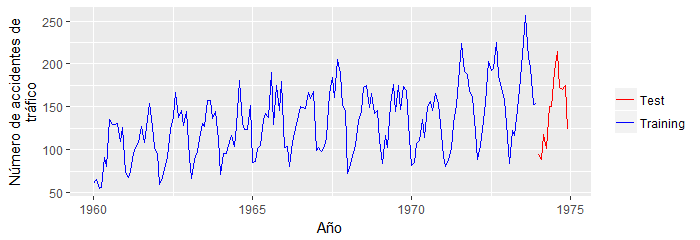
\includegraphics[scale = 0.7]{Images/Modelizacion/31.png}}
    \caption{Accidentes de tráfico ocurridos en Ontario en el periodo 1960-1975}
    \label{accidentes}
\end{figure}

\section{Forecast Package}
Esta librería está conformada por métodos orientados al análisis de series temporales univariantes, ya sea desde un punto de vista más clásico o desde uno más orientado a modelos del tipo ARIMA. Además incluye también algunos modelos de predicción algo más avanzados \cite{forecast}.

Esta vez vamos a utilizar la librería $\verb!rdatamarket!$ para importar a través de una API los datos en formato $\verb!zoo!$ directamente de la web de \textit{datamarket} \cite{datamarket}.

Esta librería es capaz de trabajar con cualquier tipo de objeto temporal pero personalmente recomiendo $\verb!ts!$ ya que en ocasiones se apoya en métodos de la librería $\verb!stats!$ para construir los distintos modelos. Aun así, como ya hemos visto en el apartado anterior, no suele haber problemas entre conversiones $\verb!ts!$ y $\verb!zoo!$. El código correspondiente a esta libreria se muestra en el Anexo III.

\subsection{Preprocesado}
En ocasiones nos puede resultar útil encontrar los periodos estacionales dominantes en nuestra serie, para ello podemos recurrir a $\verb!findfrequency()!$, un método que automáticamente nos devolverá el periodo estacional de nuestra serie, en nuestro caso es 12 (se presentan periodos cada 12 meses, es decir, cada año).

Un método muy útil para estudiar la estacionalidad es $\verb!seasonplot()!$. Con él vamos a poder representar gráficamente cada año (periodo estacional) por separado y comparar cómo evoluciona la estacionalidad a medida que pasa el tiempo. Su sintaxis es la siguiente:
\begin{Verbatim}[fontsize=\footnotesize]
seasonplot(x, s, …)
\end{Verbatim}

En el que $\verb!x!$ es la serie temporal a representar y $\verb!s!$ el periodo estacional. Una opción es introducir al argumento $\verb!s!$ la función $\verb!findfrequency()!$ aplicada a nuestra serie para que automáticamente utilice este periodo estacional. En la Figura \ref{season} se muestra el gráfico originado por este método correspondiente a nuestra serie $\verb!acc.train!$. En él se puede apreciar como el menor número de accidentes se registran a principio de año y este se va incrementando hasta que alcanza su máximo en los meses de verano, después disminuye en comparación con la primera mitad del año pero sigue mostrando valores altos en los últimos meses del año.
\begin{figure}
    \centering
    \centerline{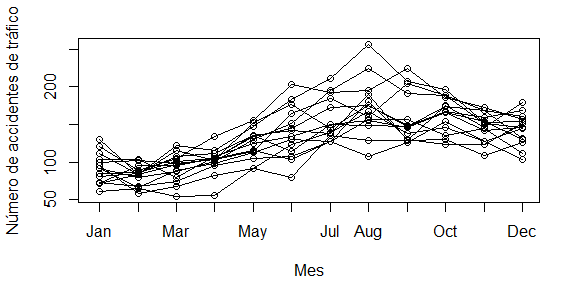
\includegraphics[scale = 0.7]{Images/Modelizacion/32.png}}
    \caption{Representación anual de la estacionalidad de la serie}
    \label{season}
\end{figure}

Vamos a descomponer nuestra serie con el método $\verb!decompose!$ de la librería $\verb!stats!$ y vamos a guardar el resultado en $\verb!acc.train.decomp!$. A través de los métodos $\verb!seasonal()!$, $\verb!trendcycle()!$ y $\verb!remainder()!$ vamos a poder extraer cada una de las componentes sin necesidad de hacer \textit{subsetting} del objeto generado por $\verb!decompose!$. Hemos supuesto que nuestra serie es multiplicativa ya que parece que el nivel estacional varía con el tiempo. En la Figura \ref{descompose} se muestra el resultado de esta descomposición.
\begin{figure} [t]
\begin{subfigure}{.5\textwidth}
  \centering
  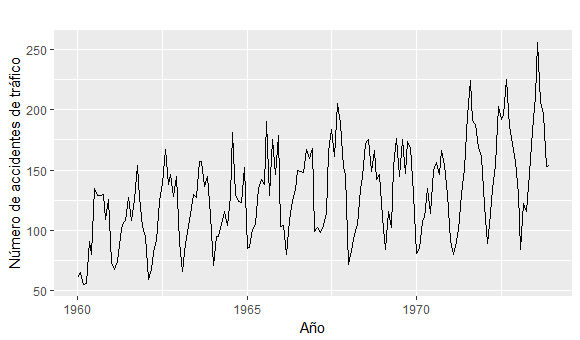
\includegraphics[width=.8\linewidth]{Images/Modelizacion/33-serie.png}
  \caption{Serie original}
  \label{fig:sfig1}
\end{subfigure}
\begin{subfigure}{.5\textwidth}
  \centering
  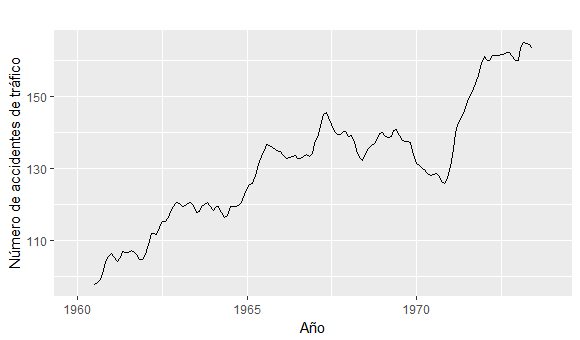
\includegraphics[width=.8\linewidth]{Images/Modelizacion/33-tend.png}
  \caption{Tendencia}
  \label{fig:sfig2}
\end{subfigure}
\begin{subfigure}{.5\textwidth}
  \centering
  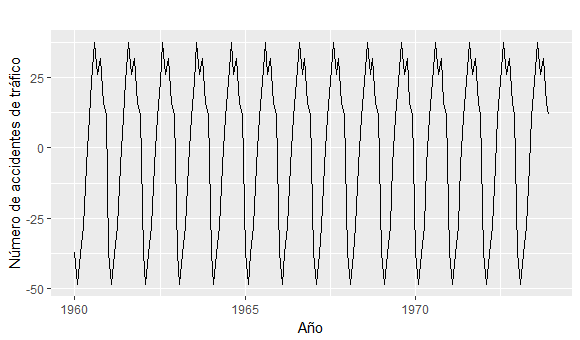
\includegraphics[width=.8\linewidth]{Images/Modelizacion/33-season.png}
  \caption{Estacionalidad}
  \label{fig:sfig1}
\end{subfigure}
\begin{subfigure}{.5\textwidth}
  \centering
  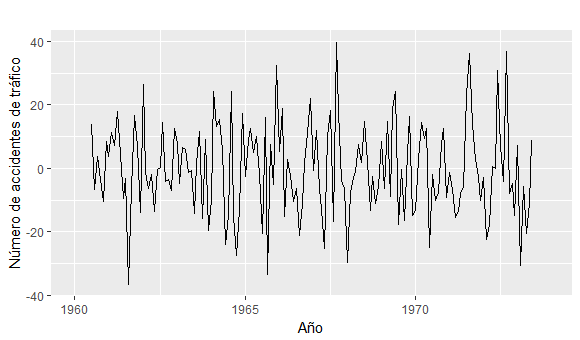
\includegraphics[width=.8\linewidth]{Images/Modelizacion/33-irre.png}
  \caption{Irregular}
  \label{fig:sfig2}
\end{subfigure}
\caption{Descomposición de la serie \PVerb{acc.train}}
\label{descompose}
\end{figure}

Para ver si realmente esta descomposición recoge todos los aspectos deterministas de la serie vamos a estudiar los residuos a través del método $\verb!Box.test!$ de la librería $\verb!stats!$. Este método implementa el test de Ljung-Box a nuestros residuos para contrastar la hipótesis nula de independencia entre observaciones. Obtenemos un p-valor de 0.7658 por lo que parece que esta descomposición recoge una parte importante de los patrones deterministas del proceso que genera nuestra serie ya que la componente aleatoria es ruido.

En la Figura \ref{descompose} se puede apreciar como la componente estacional se mantiene constante a lo largo del tiempo por lo que podría tener sentido eliminarla de la serie. Para ello recurrimos a $\verb!seasadj()!$. El resultado tras aplicar este método se muestra en la Figura \ref{deses}.
\begin{figure}
    \centering
    \centerline{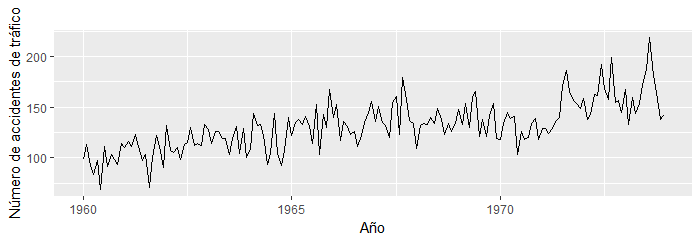
\includegraphics[scale = 0.7]{Images/Modelizacion/34.png}}
    \caption{Serie desestacionalizada}
    \label{deses}
\end{figure}

En ocasiones es muy importante saber si una serie es estacionaria o no, para ello se suelen recurrir a distintos test estadísticos de la raíz unitaria. En esta librería recomiendo el método $\verb!ndiffs()!$ con el cual se obtiene el número de diferenciaciones a aplicar a nuestra serie para que sea estacionaria. Si la salida es 0 significa que nuestra serie es estacionaria, en caso contrario no lo es. Su sintaxis es la siguiente:
\begin{Verbatim}[fontsize=\footnotesize]
ndiffs(x, alpha = 0.05, test = c("kpss", "adf", "pp"), max.d = 2)
\end{Verbatim}

Este método devuelve el número de veces que se ha tenido que diferenciar nuestra serie para asegurar la hipótesis de estacionariedad del test especificado a través de $\verb!test!$ a un nivel de significación introducido en $\verb!alpha!$. Nosotros usaremos el test aumentado de Dickey Fuller (ADF). Obtenemos una salida de 0 por lo que parece que no es necesario diferenciar la serie para trabajar bajo estacionariedad.

Al igual que en otras librerías es posible estudiar más en profundidad la tendencia a partir del método $\verb!ma()!$ encargado de aplicar un suavizado de medias móviles. En este caso tiene sentido suavizar la serie con un orden 12 para conseguir así sumarizar los datos anualmente eliminando la influencia de la estacionalidad, pudiéndose apreciar de forma más clara la evolución general de la serie.

\subsection{Modelos ingenuos}
El preprocesado de los datos temporales es importante pero como bien se puede apreciar en su propio nombre ($\verb!forecast!$) esta librería se centra en la predicción a través de modelos temporales. Estos modelos tienen sus propios métodos capaces de aportarnos información relevante para el correcto ajuste y predicción del modelo aplicado. Comenzaremos aplicando y estudiando los resultados de algunos modelos de predicción más sencillos.

Estos modelos sencillos o ingenuos se utilizan para trabajar bajo el principio de parsimonia. Bajo este principio conseguimos controlar la relación esfuerzo-resultado, evitando así destinar muchos recursos al ajuste de modelos complejos que apenas mejoran las predicciones de uno ingenuo.

El primer modelo ingenuo es el provisto por el método $\verb!meanf()!$ y consiste en simplemente predecir los valores de la serie a partir de su media. Su sintaxis es la siguiente:
\begin{Verbatim}[fontsize=\footnotesize]
meanf(y, h, level = c(80, 95), …)
\end{Verbatim}

\noindent donde $\verb!y!$ es un vector numérico o en nuestro caso una serie temporal, $\verb!h!$ es el número de periodos que deseamos predecir y $\verb!level!$ es el nivel de confianza de las predicciones realizadas. El objeto generado es de la clase $\verb!forecast!$ y nos aporta una gran cantidad de información útil para realizar diagnósticos de nuestro modelo (predicciones, residuales, serie original, etc…).

A continuación se muestra como ajustar un modelo ingenuo de estas características a la serie $\verb!acc.train!$ que se encargue de predecir los valores para el año 1974:

\begin{Verbatim}[fontsize=\footnotesize, numbers = left]
model <- meanf(acc.train, h = 12)
autoplot(model)
\end{Verbatim}

En la Figura \ref{meanf_1} generada por el código anterior se muestra la serie utilizada para entrenar al modelo y los resultados de la predicción. En este caso la predicción para el año 1974 es una línea recta ya que estamos utilizando únicamente la media. La franja azul clara representa el intervalo de confianza a un nivel del 95$\%$ y la más oscura al 80$\%$. La Figura \ref{comp} nos permite comparar gráficamente la predicción con los valores reales.
\begin{figure}
    \centering
    \centerline{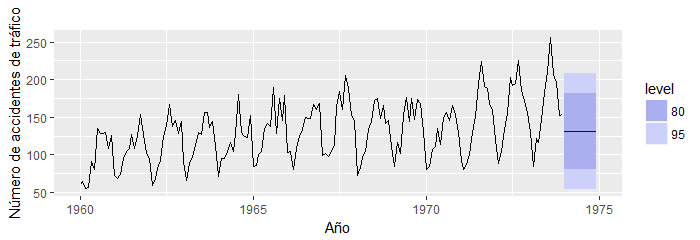
\includegraphics[scale = 0.7]{Images/Modelizacion/35.png}}
    \caption{Predicción del modelo correspondiente a \PVerb{meanf()}}
    \label{meanf_1}
\end{figure}

Inspeccionar gráficamente el ajuste del modelo no es siempre la mejor opción ya que en muchas ocasiones necesitaremos medidas más objetivas para, por ejemplo, comparar entre modelos. Esta librería incorpora un método muy útil conocido como $\verb!accuracy()!$. Su sintaxis es la siguiente:
\begin{Verbatim}[fontsize=\footnotesize]
accuracy(f, x, …)
\end{Verbatim}

A través del argumento $\verb!f!$ se introduce el modelo a evaluar almacenado en un objeto de clase $\verb!forecast!$. El argumento $\verb!x!$ es opcional, en él se introduce el conjunto de test en caso de que se disponga de uno. En nuestro caso vamos a pasar el método $\verb!accuracy()!$ a nuestro modelo \PVerb{model} y al conjunto de \textit{test} $\verb!acc.test!$. La salida resultante es la siguiente:
\begin{Verbatim}[fontsize=\footnotesize]
                       ME     RMSE      MAE        MPE
Training set 5.392491e-15 38.73302 31.48058 -10.085477
Test set     1.439286e+01 41.43521 36.28770   2.639993
                     MAPE     MASE      ACF1 Theil's U
                 27.71539 1.774836 0.7359523        NA
                 25.15689 2.045855 0.6310518  1.205019
\end{Verbatim}

Estamos obteniendo varias medidas de precisión tanto para el conjunto de \textit{training} como para el de \textit{test}. Nosotros nos centraremos en las dos siguientes:

\begin{description}
  \item[$\bullet$ RMSE:]Raíz del error cuadrático medio.
    \begin{equation}
    RMSE = \sqrt{\frac{1}{T} \sum_{i = 1}^{n}(Y_i - \widehat{Y}_i)^2}
    \end{equation}
  \item[$\bullet$ MAE:]Error medio absoluto.
  \begin{equation}
    MAE = \frac{1}{T} \sum_{i = 1}^{n} \lvert Y_i - \widehat{Y}_i \lvert
  \end{equation}
\end{description}

La MAE es muy común en las distintas competiciones de \textit{Data Science} que se realizan en Internet.

En nuestro modelo estamos obteniendo un RMSE y un MAE para el conjunto de \textit{training} de 38.73302 y 31.48058, respectivamente. Para el conjunto de \textit{test} obtenemos 41.43521 y 36.28770. En ambos conjuntos obtenemos errores similares (siendo mayores los del \textit{test}) lo cual es una buena señal. El MAE es fácilmente interpretable: en este caso significa que estamos errando en 36 accidentes mortales en promedio en nuestras predicciones.

Otro método muy útil incluido en esta librería es $\verb!checkresiduals()!$. Con él vamos a poder estudiar los residuos de los modelos ajustados ya que nos va a ofrecer su gráfico, su correlograma, su histograma y un test estadístico para contrastar la significatividad de las autocorrelaciones. Su sintaxis es la siguiente:
\begin{Verbatim}[fontsize=\footnotesize]
checkresiduals(object, lag, test, ...)
\end{Verbatim}

A través del argumento $\verb!object!$ vamos a introducir el modelo a evaluar, $\verb!lag!$ fija los rezagos a utilizar en el test estadístico y $\verb!test!$ el propio test que puede ser el de Ljung-Box o el de Breusch-Godfrey. Por defecto el método selecciona automáticamente el test de Breusch-Godfrey si el modelo a evaluar es de regresión, en caso contrario utiliza el de Ljung-Box.

En el caso de nuestro modelo ingenuo estamos obteniendo un p-valor para el test de Ljung-Box de prácticamente cero por lo que parece haber aún relaciones y patrones en los residuos.  Esto es algo lógico ya que la media es incapaz de recoger ningún patrón importante de los datos. Los gráficos resultantes se muestran en la Figura \ref{checkresiduals}.
\begin{figure}
    \centering
    \centerline{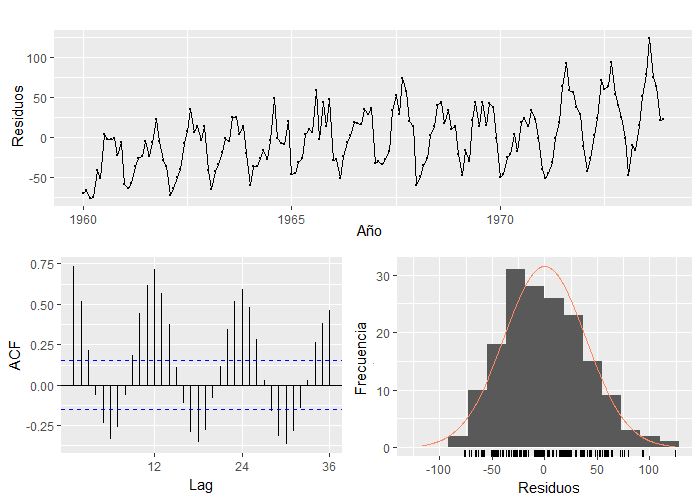
\includegraphics[scale = 0.7]{Images/Modelizacion/37.png}}
    \caption{Resultado del método \PVerb{checkresiduals()}}
    \label{checkresiduals}
\end{figure}

Es posible también utilizar el último valor observado para predecir los nuevos valores de la serie, el método $\verb!naive()!$ se encarga de implementar esto. La sintaxis es idéntica a la del método anterior y los resultados también, solo que en este caso la línea formada por los valores predichos está desplazada hacia arriba (el último valor de la serie es mayor que la media). Este resultado se muestra en la Figura \ref{comp}.

Obtenemos un RMSE y un MAE en el conjunto de \textit{test} de 39.73873 y 33.8333, respectivamente. Son unos resultados muy similares a los obtenidos por $\verb!meanf()!$ por lo que apenas hay diferencias entre ambos modelos. En este caso los residuos también parecen mostrar de forma significativa autocorrelaciones.

A través del método $\verb!rwf()!$ es posible ajustar una variante del modelo ingenuo provisto por $\verb!naive()!$ conocido como caminata aleatoria con deriva. Teóricamente se define como:
\begin{equation}
    Y_t = \delta + Y_{t - 1} + a_t
\end{equation}

\noindent por lo que realizaremos la predicción de $Y_{t + h}$ a partir de:
\begin{equation}
    \widehat{Y}_{t + h} = \delta h + \widehat{Y}_{t + h - 1}
\end{equation}

La deriva $\delta$ refleja el cambio medio de la serie a lo largo del tiempo y se calcula de la siguiente manera:
\begin{equation}
    \delta = \bigg( \frac{Y_T - Y_1}{T - 1} \bigg)
\end{equation}

Para incluir esta deriva es necesario pasar al argumento $\verb!drift!$ el valor de $\verb!TRUE!$, en caso contrario obtendremos los mismos resultados que con $\verb!naive()!$. En la Figura \ref{comp} se puede apreciar como en este caso las predicciones no forman una línea totalmente horizontal sino que presentan una pequeña pendiente gracias a la inclusión de la deriva. Obtenemos unas medidas de precisión prácticamente idénticas al modelo sin deriva y unos residuos correlacionados entre sí. Todo esto es lógico ya que la inclusión de la deriva no supone un mejor ajuste, nos falta algo a tener en cuenta en el modelo para lograr ajustes aceptables.

Como bien hemos comentado, esta serie muestra una componente estacional muy marcada por lo que una opción sería ajustar un modelo que predijese de acuerdo a los valores estacionales del periodo anterior, en este caso del año anterior. Esto es lo que ofrece $\verb!snaives()!$ que en vez de predecir con el valor inmediatamente anterior predice con el correspondiente al periodo estacional anterior, por ejemplo si queremos predecir el valor de nuestra serie en julio de 1974 este recurrirá al valor en julio de 1973. Más formalmente se define como:
\begin{equation}
    Y_t = Y_{t - M} + a_t
\end{equation}

\noindent siendo M el periodo estacional presente en la serie, en nuestro caso 12. En la Figura \ref{snaives} se observa como efectivamente lo único que hemos hecho ha sido predecir el año 1974 a partir del 1973. Aunque este método parece sencillo obtenemos un RMSE y un MAE de 25.98237 y 22.58333 respectivamente. Esto significa que estamos consiguiendo obtener un ajuste relativamente bueno, esto se debe a que esta serie parece mostrar un comportamiento estacional bastante estable en los últimos años estudiados. Sin embargo no es suficiente ya que el test de Ljung-Bbox nos dice que aún existen correlaciones entre los residuos, necesitamos algo más avanzado.
\begin{figure}
    \centering
    \centerline{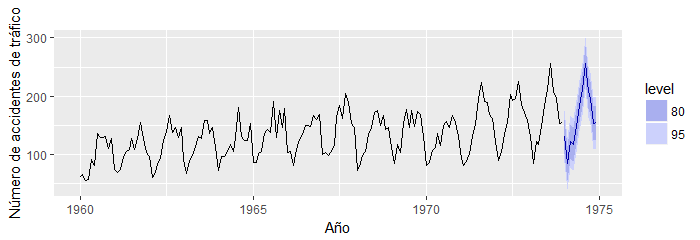
\includegraphics[scale = 0.7]{Images/Modelizacion/310.png}}
    \caption{Predicción del modelo correspondiente a \PVerb{snaives()}}
    \label{snaives}
\end{figure}

\begin{figure}
    \centering
    \centerline{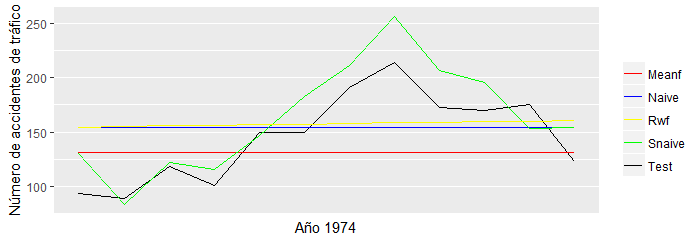
\includegraphics[scale = 0.7]{Images/Modelizacion/311.png}}
    \caption{Comparación de los modelos ingenuos con el \textit{test}}
    \label{comp}
\end{figure}

\subsection{Modelo lineal}
A continuación vamos a manejar algunos modelos más completos a fin de conseguir un mejor ajuste. Comenzaremos ajustando un modelo de regresión lineal con la tendencia y la estacionalidad como variables independientes:
\begin{equation}
    Y_{t} = \beta_0 + \beta_1 t + \sum_{i = 2}^{M} \lambda_i d_i
\end{equation}

\noindent donde $d_i$ son variables dummy que toman el valor 1 cuando $i = m$ con $m \neq 1$ siendo $m$ el periodo al que corresponde $Y_t$. Los coeficientes $\lambda_i$ se interpretan como el cambio medio correspondiente al periodo estacional $i$. Para ajustar este tipo de modelos recurriremos al método $\verb!tslm()!$. Este método funciona de la misma manera que $\verb!lm()!$, solo que nos permite añadir y calcular las variables independientes correspondientes a la tendencia y a la estacionalidad de forma mucho más sencilla. A continuación se muestra el código para ajustar este modelo a nuestros datos pudiendo así predecir un año:
\begin{Verbatim}[fontsize=\footnotesize, numbers = left]
model <- tslm(acc.train ~ trend + season)
pred <- forecast(model, h = 12)
\end{Verbatim}

La sintaxis seguida es la utilizada en $\verb!lm()!$, es decir, estamos ajustando un modelo de regresión con $\verb!acc.train!$ como variable dependiente y $\verb!trend!$ y $\verb!season!$ como independientes (estas variables son calculadas internamente por el propio método). En este caso el método $\verb!tslm()!$ no nos generará un objeto $\verb!forecast!$ sino $\verb!lm!$ por lo que necesitamos transformarlo mediante $\verb!forecast()!$ introduciendo como argumentos el modelo y el número de observaciones a predecir.

A través del \textit{subsetting} $\verb!$coefficients!$ es posible acceder a los coeficientes de nuestro modelo. El modelo final ajustado es el siguiente:
\begin{equation}
    \widehat{Y}_{t} = 63.75 + 0.35 t - 9.99 d_2 - 0.06 d_3 + 8.72 d_4 + ... + 47.88 d_{12}
\end{equation}

El resultado de la predicción se muestra en la Figura \ref{tslm}. Estamos obteniendo un MAE de 19.44597 que es el mejor hasta el momento, sin embargo seguimos teniendo correlaciones entre los residuos por lo que parece que este modelo no acaba de recoger todas las relaciones presentes en nuestra serie.
\begin{figure}
    \centering
    \centerline{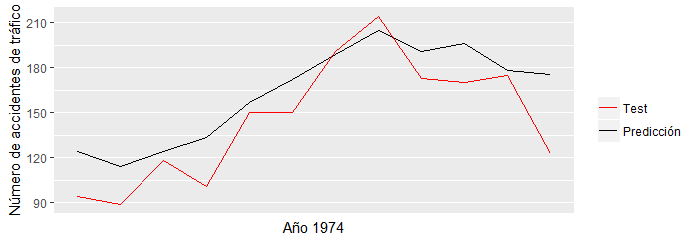
\includegraphics[scale = 0.7]{Images/Modelizacion/312.png}}
    \caption{Comparación de las predicciones realizadas por \PVerb{tslm()} con el \textit{test}}
    \label{tslm}
\end{figure}

\subsection{Triple suavizado exponencial}
Los modelos de suavizado exponencial pueden parecer simples a primera vista pero en ocasiones consiguen realizar predicciones bastante acertadas. Nuestra serie presenta tendencia y estacionalidad por lo que es posible modelizarla a través de un triple suavizado exponencial o Holt-Winters, con coeficientes $\alpha$, $\beta$ y $\gamma$. La idea es aplicar un suavizado exponencial ponderado a la componente estacional, al nivel y a la tendencia

Este modelo está compuesto por tres ecuaciones de suavizado y una de predicción. Estas tres ecuaciones estiman individualmente el nivel $l_t$ (el valor suavizado de la serie), la tendencia $b_t$ y la estacionalidad $S_t$. Estos tres componentes se relacionan en la ecuación de predicción para obtener el valor estimado. A continuación se muestra el modelo para el caso aditivo:
\begin{align}
  \widehat{Y}_{t+h} &= l_t + h b_t + S_{t - M + h^+_M} \\
  l_t &= \alpha(Y_t - S_{t - M}) + (1 -\alpha)(l_{t-1}+ b_{t-1}) \\
  b_t &= \beta(l_t - l_{t-1}) + (1 -\beta) b_{t-1} \\
  S_t &= \gamma(Y_t - l_{t-1} + b_{t-1}) + (1 - \gamma) S_{t-M}
\end{align}

\noindent donde $h^+_M = \floor{(h - 1) \quad mod \quad M} + 1$. Esto nos asegura que las estimaciones estacionales para cierto índice provienen del último año observado y no del predicho. Como se puede apreciar en el modelo aditivo la estacionalidad se presenta en términos absolutos mientras que en el multiplicativo se presenta en términos relativos (porcentajes). A continuación se muestra el modelo correspondiente al supuesto multiplicativo:
\begin{align}
  \widehat{Y}_{t+h} &= (l_t + h b_t) S_{t - M + h^+_M} \\
  l_t &= \alpha \frac{Y_t}{S_{t-M}} + (1 -\alpha)(l_{t-1}+ b_{t-1}) \\
  b_t &= \beta(l_t - l_{t-1}) + (1 -\beta) b_{t-1} \\
  S_t &= \gamma \frac{Y_t}{(l_{t-1} + b_{t-1})} + (1 - \gamma) S_{t-M}
\end{align}

Los coeficientes $\alpha$, $\beta$ y $\gamma$ determinan la influencia de las tres componentes en las estimaciones. Están comprendidos entre 0 y 1, cuanto más cerca estén de cero más importancia darán a las observaciones alejadas en el tiempo y viceversa. Aunque es posible elegir estos coeficientes manualmente lo más común es calcularlos mediante métodos de optimización basados en la minimización de la suma de los cuadrados de los residuos.

Si nos fijamos en las ecuaciones (53) y (57) podemos apreciar que la tendencia es constante, es decir, no para de crecer (o decrecer) con el tiempo. Esto no suele ofrecer buenos resultados pues la realidad no es así, por ello surgió la tendencia amortiguada (\textit{damped trend}) que consigue suavizar en el tiempo la evolución de la tendencia. Para ello debemos añadir un nuevo coeficiente $\phi$ conocido como parámetro de amortiguación (\textit{damping parameter}). En el caso aditivo tendríamos lo siguiente (el caso multiplicativo se muestra en el Anexo IV).
\begin{align}
  \widehat{Y}_{t+h} &= l_t + (\phi + \phi^2 + ... + \phi^h)b_t + S_{t - M + h^+_M} \\
  l_t &= \alpha(Y_t - S_{t - M}) + (1 -\alpha)(l_{t-1}+ \phi b_{t-1}) \\
  b_t &= \beta(l_t - l_{t-1}) + (1 -\beta) \phi b_{t-1} \\
  S_t &= \gamma(Y_t - l_{t-1} + \phi b_{t-1}) + (1 - \gamma) S_{t-M}
\end{align}

\noindent donde $0 < \phi < 1$. Si $\phi = 1$ el modelo no varía respecto al original, en caso contrario las predicciones realizadas a corto plazo tienen una tendencia mucho más marcada que las de largo plazo \cite{hyndman2014forecasting}.

En esta librería el método $\verb!hw()!$ se encarga de implementar este modelo, su sintaxis es la siguiente:
\begin{Verbatim}[fontsize=\footnotesize]
hw(y, h = 2*frequency(x), seasonal = c("additive", "multiplicative"),
   damped = FALSE, initial = c("optimal", "simple"), alpha = NULL,
   beta =  NULL, gamma = NULL, phi = NULL, …)
\end{Verbatim}

A través de $\verb!y!$ introducimos la serie sobre la que vamos a trabajar y en el argumento $\verb!h!$ indicaremos el número de predicciones a realizar. Dependiendo de nuestra serie aplicaremos el modelo aditivo o multiplicativo que indicaremos a través de $\verb!seasonal!$. Si queremos trabajar con la tendencia amortiguada pasaremos $\verb!damped!$ como $\verb!TRUE!$. Al ser un modelo recursivo necesitamos iniciar de alguna manera las distintas componentes, recomiendo utilizar $\verb!optimal!$. Es posible fijar manualmente los valores de los coeficientes del modelo a través de los argumentos homónimos. A continuación ajustaremos este modelo a nuestros datos y a través de $\verb!summary()!$ estudiaremos sus características principales:
\begin{Verbatim}[fontsize=\footnotesize, numbers = left]
model <- hw(acc.train, h = 12, damped = TRUE, seasonal = "multiplicative",
            initial = "optimal")
summary(model)
\end{Verbatim}

Estamos ajustando un triple suavizado exponencial con tendencia amortiguada y suponiendo multiplicatividad. El coeficiente $\alpha$ tiene un valor de 0.1708 y $\beta$ y $\gamma$ prácticamente de cero, esto significa que se está teniendo muy en cuenta los valores pasados de la serie, sobre todo para la tendencia y la estacionalidad. El coeficiente de amortiguación $\phi$ toma el valor de 0.9623 por lo que la amortiguación de la tendencia ocurre a muy largo plazo. El $\verb!summary()!$ nos muestra también los valores iniciales de las tres componentes y las predicciones con los intervalos al 80$\%$ y 95$\%$.

En la  Figura \ref{hw_fit} se muestran los datos originales junto al ajuste generado por este modelo bajo supuestos de aditividad y multiplicatividad. También se muestran en la Figura \ref{hw_pred} las predicciones de ambos modelos para el año 1974 junto a los valores reales. Para el modelo aditivo obtenemos un MAE de 19.67722 y para el multiplicativo 15.04762 por lo que nos quedaremos con este último. Es el más bajo hasta el momento por lo que parece que este modelo se puede usar con bastante seguridad como predictor de los accidentes de tráfico en Ontario, sin embargo aún tenemos información relevante en los residuos ya que el p-valor para el test de Ljung-Box es prácticamente cero.
\begin{figure}
    \centering
    \centerline{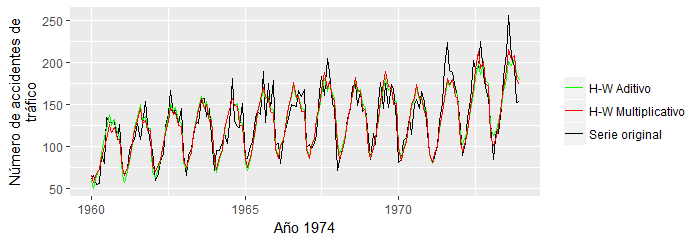
\includegraphics[scale = 0.7]{Images/Modelizacion/313.png}}
    \caption{Distintos ajustes de \PVerb{hw()}}
    \label{hw_fit}
\end{figure}

\begin{figure}
    \centering
    \centerline{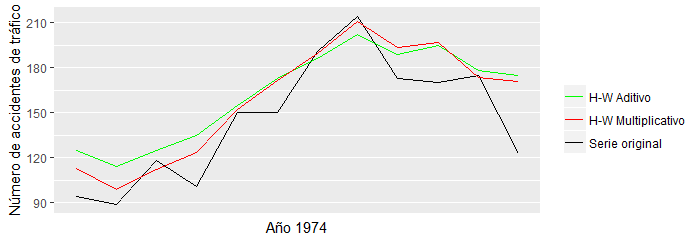
\includegraphics[scale = 0.7]{Images/Modelizacion/314.png}}
    \caption{Predicciones de los modelos correspondientes a \PVerb{hw()}}
    \label{hw_pred}
\end{figure}

\subsection{Red neuronal}
Son bien conocidas en el ámbito de la modelización las redes neuronales artificiales. Estos algoritmos consiguen adaptarse a una gran variedad de problemas debido a su característica estructura capaz de imitar el cerebro humano. Están estructuradas en capas formadas por unidades de procesamiento individual conocidas como neuronas. Estas están conectadas entre sí a través de conexiones ponderadas. La predicción realizada por la red dados unos \textit{inputs} determinados se obtiene en su capa final conocida como capa de salida. Estos algoritmos son realmente complejos, por ello nosotros nos centraremos únicamente en uno aplicado a series temporales univariantes.

En esta librería existe un método realmente útil encargado de implementar este tipo de redes neuronales conocido como $\verb!nnetar()!$.  Este método implementa una red \textit{feed-forward} con una única capa oculta o intermedia compuesta por $k$ neuronas. Toma como \textit{inputs} los últimos $p$ valores de la serie los cuales utiliza para realizar la predicción, estos valores obviamente van a estar rezagados respecto al que se busca predecir. Como este modelo también se apoya en modelos autorregresivos se conoce como \textit{Neural Network Auto Regressive  Model} y su notación es NNAR$(p, k)$.

Existe una pequeña variación de este modelo destinada a datos estacionales  que incluye además como \textit{inputs} los correspondientes valores en periodos anteriores de la observación a predecir, este modelo tiene la forma NNAR$(p, P, k)_M$ donde $M$ es la periodicidad de la serie y $P$ es el número de periodos anteriores de los que tomamos las observaciones como \textit{input}, es decir, en este caso tenemos una red con $k$ neuronas en su capa intermedia y con los siguientes \textit{inputs}:
\begin{equation}
    Y_{t-1}, Y_{t-2},...,Y_{t-p}, Y_{t-M}, Y_{t-2M},...,Y_{t-PM}
\end{equation}

Este método pertenece a la familia del método $\verb!nnet()!$ incluido en la librería $\verb!nnet!$ por lo que ambas comparten algunos argumentos. La sintaxis de $\verb!nnetar()!$ es la siguiente:
\begin{Verbatim}[fontsize=\footnotesize]
nnetar(y, p, P = 1, size, repeats = 20, decay, ...)
\end{Verbatim}

A través del argumento $\verb!y!$ se introduce la serie a modelizar y por $\verb!p!$ y $\verb!P!$ los parámetros ya comentados. El argumento $\verb!size!$ se corresponde con $k$, es decir, el número de neuronas que conforman la capa oculta. El entrenamiento de la red consiste en estimar los pesos que ponderan las conexiones entre neuronas, estos pesos se van actualizando a medida que le vamos pasando observaciones de la serie durante el entrenamiento por lo que es necesario iniciarles aleatoriamente. Para evitar la influencia de la aleatoriedad en los resultados se entrenan varias redes cada una con unos pesos iniciales distintos y se utiliza las media de las predicciones de todas ellas como predicción final. Este número de redes se introduce al modelo a través del argumento $\verb!repeats!$.

A continuación se ajusta una red neuronal con todos los argumentos por defecto y se predice el año 1974 de nuestra serie:
\begin{Verbatim}[fontsize=\footnotesize, numbers = left]
model <- nnetar(acc.train)
pred <- forecast(model, h = 12)
summary(model)
\end{Verbatim}

Observando los valores de los parámetros de nuestro modelo observamos que ha seleccionado $p = 1$, $P = 1$ y $k = 1$, por lo que parece que la estructura de nuestra red es bastante sencilla. El RMSE y el MAE en el conjunto de \textit{test} son 31.971323 y 26.22965 respectivamente, sin embargo en el conjunto de \textit{training} toman los valores 4.062094 y 3.12345. Esta diferencia es un indicador de que algo está fallando. En este tipo de modelos enmarcados dentro del \textit{machine learning} se suele dar con frecuencia un problema bastante común conocido como \textit{overfitting} causado por un sobreajuste del modelo en el conjunto de \textit{training} que hace que la inferencia sobre el conjunto de \textit{test} sea pésima. Para evitar esto se suele introducir un parámetro de regularización que limita al modelo obligándolo a suavizar su ajuste sobre el conjunto de \textit{training} para así poder obtener unas mejores inferencias. Este parámetro se introduce a partir del argumento $\verb!decay!$.

Para saber qué valor dar al parámetro de regularización  vamos a estudiar su comportamiento, para ello vamos a ejecutar varios modelos con valores de $\verb!decay!$ distintos y vamos a estudiar su MAE. En la Figura \ref{decay} se puede apreciar como el MAE desciende a medida que aumenta el parámetro de regularización, sin embargo cuando el parámetro toma valores cercanos a 9 comienza a estabilizarse, esto significa que el valor idóneo de este parámetro está entre 9 y 10. Si ajustamos una red con un decay de 9.5 obtenemos un RMSE y MAE en el conjunto de \textit{test} de 17.41186 y 14.86415 respectivamente, el mejor hasta el momento. Parece que hemos solucionado el \textit{overfitting} del modelo anterior ya que para el conjunto de \textit{training} obtenemos unos valores de 19.84883 y 15.51073.
\begin{figure}
    \centering
    \centerline{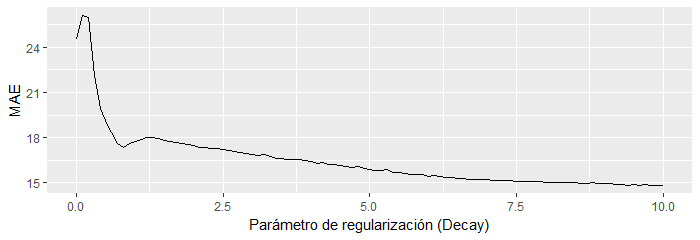
\includegraphics[scale = 0.7]{Images/Modelizacion/315.png}}
    \caption{Evolución del MAE respecto a \PVerb{decay}}
    \label{decay}
\end{figure}

Es posible mejorar el modelo introduciendo manualmente el resto de argumentos al método. Estudiando la evolución de los distintos parámetros de la misma forma (Anexo V) hemos llegado a la conclusión de que el modelo óptimo es el siguiente:
\begin{Verbatim}[fontsize=\footnotesize]
model <- nnetar(acc.train, repeats = 25, size = 20, decay = 9.5, p = 20, P = 4)
\end{Verbatim}

Obtenemos un MAE para el conjunto de test de 13.29118, el más bajo hasta el momento por lo que tiene sentido utilizar este modelo para predecir los accidentes de tráfico. En la Figura \ref{red} se muestra gráficamente el ajuste y se puede apreciar esa suavización de la predicción causada por el parámetro de regularización.
\begin{figure}
    \centering
    \centerline{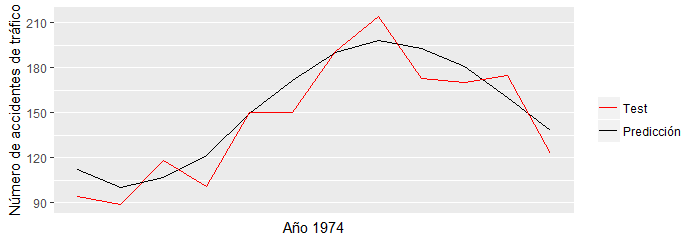
\includegraphics[scale = 0.7]{Images/Modelizacion/317.png}}
    \caption{Comparacións de la red óptima con el \textit{test}}
    \label{red}
\end{figure}

\subsection{Modelos ARIMA}
Los modelos ARIMA se utilizan con mucha frecuencia en la modelización de series temporales aunque, como ya se ha explicado, necesitan trabajar bajo unos supuestos más estrictos.

Uno de estos supuestos es el de homogeneidad de la varianza. Si la varianza de nuestra serie no se mantiene constante en el tiempo estaremos ante una serie no estacionaria y necesitaremos realizar algunas transformaciones a fin de poder aplicar esta clase de modelos. En la mayor parte de casos nos vale con aplicar logaritmos a nuestra serie, algo muy sencillo de hacer con $\verb!log()!$, sin embargo a veces esto no es suficiente y necesitaremos transformaciones más complejas como la de Box Cox. La librería $\verb!forecast!$ contiene un método muy bien optimizado para implementar esta transformación conocido como $\verb!BoxCox()!$. Su sintaxis es la siguiente:
\begin{Verbatim}[fontsize=\footnotesize]
BoxCox(x, lambda)
\end{Verbatim}

\noindent donde $\verb!x!$ recoge la serie a transformar y $\verb!lambda!$ el parámetro $\lambda$ que define la transformación. Este parámetro puede ser introducido manualmente por el usuario pero se suele utilizar el método $\verb!BoxCox.lambda()!$ que le selecciona automáticamente. Su sintaxis es la siguiente:
\begin{Verbatim}[fontsize=\footnotesize]
BoxCox.lambda(x, method = c("guerrero", "loglik"), lower = -1, upper = 2)
\end{Verbatim}

Recomiendo dejar todos los argumentos por defecto ya que así suele ofrecer muy buenos resultados. Para calcular nuestra serie transformada y mostrarla gráficamente bastaría con el siguiente código:
\begin{Verbatim}[fontsize=\footnotesize, numbers = left]
acc.train.trans <- BoxCox(x = acc.train, lambda = BoxCox.lambda(acc.train)
autoplot(acc.train.trans)
\end{Verbatim}

Apenas se aprecian diferencias entre las series transformadas y la original por lo que vamos a suponer que efectivamente nuestra serie es estacionaria en varianza.

Analizando visualmente la serie se puede apreciar que la tendencia no es constante sino que varía respecto al tiempo. Para cerciorarnos de esto vamos a aplicar el test de la raíz unitaria de Dickey-Fuller a través del método $\verb!ndiffs()!$. Obtenemos una salida de 1 lo que significa que es necesario diferenciar la serie una vez para sea estacionaria. Existe una variación de este método conocido como $\verb!nsdiffs()!$ orientado a comprobar si es necesario aplicar diferencias en la parte estacional del modelo, en este caso nos arroja una salida de 0 por lo que parece que no es necesario realizar ninguna diferencia a nivel estacional.

Una vez sabemos que nuestra serie es estacionaria podemos pasar a estudiar sus correspondientes correlogramas formados tanto a partir de la función de autocorrelación estándar como de la parcial. Los métodos encargados de implementar esto son $\verb!Acf()!$ y $\verb!Pacf()!$ respectivamente. Ambos comparten la misma sintaxis:
\begin{Verbatim}[fontsize=\footnotesize]
Acf(x, lag.max = NULL, ...)
\end{Verbatim}

A través de $\verb!x!$ introducimos la serie y con $\verb!lag.max!$ fijamos el número máximo de rezagos para los que calcular el correspondiente correlograma. En la Figura \ref{corr} se muestran estos correlogramas para nuestra serie diferenciada. El ACF parece mostrar correlaciones significativas para los rezagos 6, 12, 18 y 24.  Como estamos trabajando bajo un supuesto de estacionalidad anual vamos a fijar un $Q = 2$ y un $q = 0$ ya que parece no haber correlaciones significativas para la parte no estacional. El PACF no parece mostrar ninguna correlación significativa útil ni para la parte estacional ni para la no estacional por lo que vamos a fijar $p = 0$ y $P = 0$. Fijado esto el modelo a ajustar es un SARIMA$(0,1,0)(0,0,2)_{12}$ (en el Anexo VI se muestra una breve explicación de este tipo de modelos).
\begin{figure} [t]
\begin{subfigure}{.5\textwidth}
  \centering
  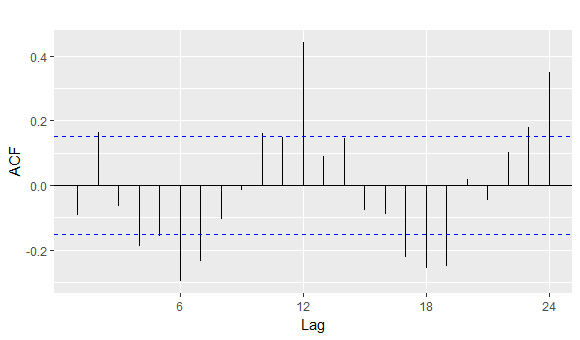
\includegraphics[width=.8\linewidth]{Images/Modelizacion/3181.png}
  \caption{ACF}
  \label{fig:sfig1}
\end{subfigure}
\begin{subfigure}{.5\textwidth}
  \centering
  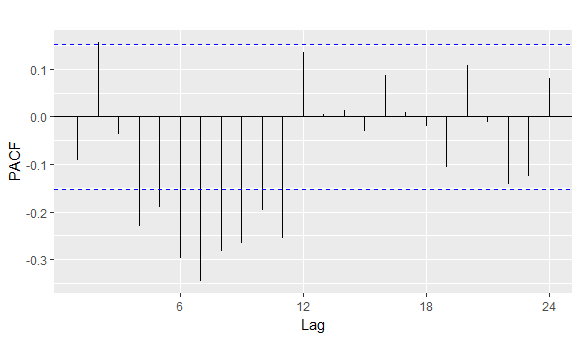
\includegraphics[width=.8\linewidth]{Images/Modelizacion/3182.png}
  \caption{PACF}
  \label{fig:sfig2}
\end{subfigure}
\caption{Correlogramas para la serie diferenciada de accidentes de tráfico en Ontario}
\label{corr}
\end{figure}

Para ajustar el modelo vamos a utilizar el método $\verb!Arima()!$ propio de esta librería y que se deriva del $\verb!arima()!$ de $\verb!stats()!$. Este método ofrece una personalización más completa del modelo además de una mejor integración con el entorno de la librería $\verb!forecast!$. Su sintaxis es la siguiente:
\begin{Verbatim}[fontsize=\footnotesize]
Arima(y, order = c(0,0,0), seasonal = c(0,0,0),
      include.mean = TRUE, include.drift = FALSE, …)
\end{Verbatim}

A través de $\verb!y!$ introducimos la serie y en $\verb!order!$ y $\verb!seasonal!$ introducimos los órdenes y las diferencias realizadas sobre cada una de las partes, respectivamente. Con el argumento $\verb!include.mean!$ se controla la inclusión del intercepto $c$ en el modelo. Si se fija como $\verb!TRUE!$ tenemos que $c \simeq \mu$ para $d = 0$ y $c = 0$ para $d > 0$. En caso de que se pase como $\verb!FALSE!$, $c = 0$ para cualquier $d$. El argumento $\verb!include.drift!$ permite también incorporar una variación de este intercepto al modelo cuando $d = 1$. El modelo generado por este método se trata de la misma forma que todos los anteriores. A continuación se muestra cómo generamos el modelo mencionado anteriormente y sus características principales:
\begin{Verbatim}[fontsize=\footnotesize, numbers = left]
model <- Arima(acc.train, order = c(0,1,0), seasonal = c(0,0,2))
summary(model)
\end{Verbatim}

La salida generada por este código es la siguiente:
\begin{Verbatim}[fontsize=\footnotesize]
          Series: acc.train
          ARIMA(0,1,0)(0,0,2)[12]

          Coefficients:
                  sma1    sma2
                0.3918  0.2472
          s.e.  0.0788  0.0739

          sigma^2 estimated as 605.1:  log likelihood=-772.19
          AIC=1550.38   AICc=1550.53   BIC=1559.73

          Training set error measures:
                              ME     RMSE      MAE       MPE
          Training set 0.3068305 24.37856 19.84998 -1.632044
                                     MAPE     MASE       ACF1
                                 15.91416 1.119117 -0.2672489
\end{Verbatim}

Con esta información tenemos que el modelo ajustado es:
\begin{equation}
    \Delta Y_t = 0.3918 \thinspace Y_{t-12} + 0.2472 \thinspace Y_{t-24} + a_t
\end{equation}

También nos ofrece unas medidas de ajuste conocidas como criterios de información. Nosotros nos centraremos en el de Akaike (AIC) ya que el resto son variaciones de este. Se calcula de la siguiente manera:
\begin{equation}
    AIC = -2 \thinspace \ln (L) + 2k
\end{equation}

\noindent donde $k$ es el número de parámetros que se han necesitado estimar y $L$ el máximo valor de la correspondiente función de verosimilitud. Estas medidas relativas son útiles ya que no solo comparan modelos de acuerdo a su ajuste sino que también penalizan por el número de parámetros estimados. En este caso tenemos que el AIC toma el valor de 1550.38. También nos muestra el MAE del conjunto de training que toma el valor de 19.84998.

Al igual que con los modelos anteriores vamos a realizar las predicciones para el año 1974 a través de $\verb!forecast()!$ y vamos a comparar a través de $\verb!accuracy()!$ los verdaderos valores ($\verb!acc.test!$) con los predichos por el modelo. Para el conjunto de test obtenemos un MAE de 22.19949 por lo que parece que no consigue igualar a algunos de los modelos ajustados anteriormente. Si estudiamos los residuos vemos que están correlacionados entre sí ya que obtenemos un p-valor para el test de Ljung Box de prácticamente cero. Esto significa que este modelo no es el óptimo ya que no consigue recoger toda la información presente en los datos.

Aunque ya hemos visto que no parecía ser necesario diferenciar la serie estacionalmente para lograr estacionariedad vamos a realizar esta diferenciación a fin de ver si el modelo que arroja ofrece mejores resultados que el anterior. Para ello vamos a aplicar a nuestra serie el método $\verb!diff()!$ con $\PVerb{lag} = 12$. En la Figura \ref{diff} se muestra la representación de la serie diferenciada junto a su correspondiente ACF y PACF.
\begin{figure}
\begin{subfigure}{.5\linewidth}
\centering
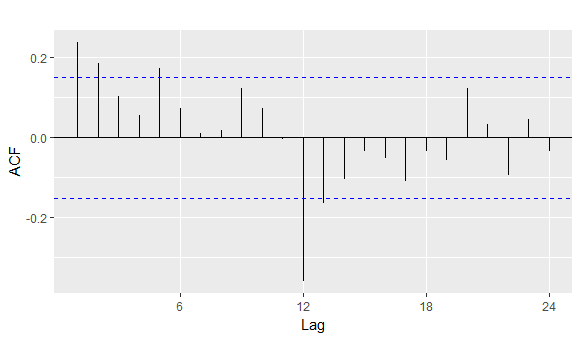
\includegraphics[width=.7\linewidth]{Images/Modelizacion/3192.png}
\caption{ACF}
\label{fig:sub1}
\end{subfigure}%
\begin{subfigure}{.5\linewidth}
\centering
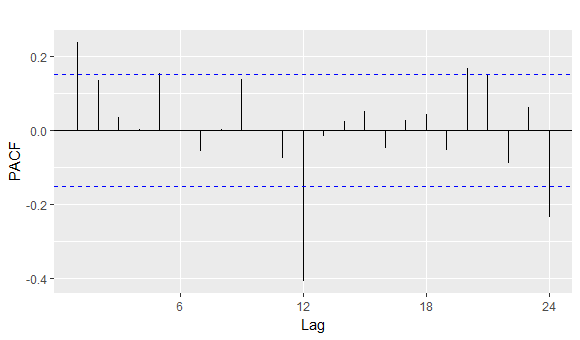
\includegraphics[width=.7\linewidth]{Images/Modelizacion/3193.png}
\caption{PACF}
\label{fig:sub2}
\end{subfigure}\\[1ex]
\begin{subfigure}{\linewidth}
\centering
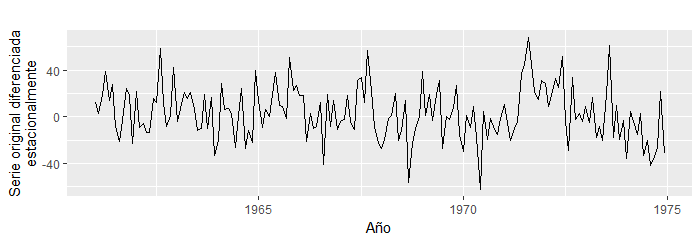
\includegraphics[width=.5\linewidth]{Images/Modelizacion/3191.png}
\caption{Serie diferenciada}
\label{fig:sub3}
\end{subfigure}
\caption{Estudio de la serie original diferenciada estacionalmente}
\label{diff}
\end{figure}

En el ACF apreciamos una correlación significativa en el primer rezago por lo que fijamos $q = 1$ y otra en el rezago 12 por lo que $Q = 1$. En el PACF ocurre lo mismo solo que en este caso también la correlación del rezago 24 parece significativa por lo que $p = 1$ y $P = 2$.

Vamos a ajustar dos modelos uno con el intercepto provisto por $\verb!include.driftt!$ y otro sin él. En la Tabla \ref{comp_1} se muestran las medidas de ajuste para ambos modelos.
\begin{table}[]
\centering
\label{my-label}
\begin{tabular}{|l|c|c|}
\hline
\multicolumn{1}{|c|}{} & \PVerb{include.drift = FALSE} & \PVerb{include.drift = TRUE} \\ \hline
AIC                    & 1367.68              & \textbf{1359.82}      \\ \hline
AICc                   & 1368.25              & \textbf{1360.58}      \\ \hline
BIC                    & 1385.98              & \textbf{1381.17}      \\ \hline
MAE en el test         & 19.22651             & \textbf{17.0999}      \\ \hline
P-valor (Ljung Box)    & 0.04321              & \textbf{0.2748}       \\ \hline
\end{tabular}
\caption{Comparación del ajuste de un SARIMA$(1,0,1)(2,1,1)_{12}$ con y sin intercepto}
\label{comp_1}
\end{table}

Se puede apreciar como el modelo con intercepto consigue mejores resultados en todos los aspectos. Tanto los criterios de información como el MAE son más bajos, además hemos conseguido que los residuos sean ruido blanco. No cabe duda de que en este caso el intercepto consigue mejorar notablemente el modelo. En la Figura \ref{comp_sarimas} se aprecia como las predicciones del modelo con $\verb!include.driftt = TRUE!$ consiguen ajustarse mejor a los valores reales gracias a la modificación en su nivel dada por la inclusión del intercepto.
\begin{figure}
    \centering
    \centerline{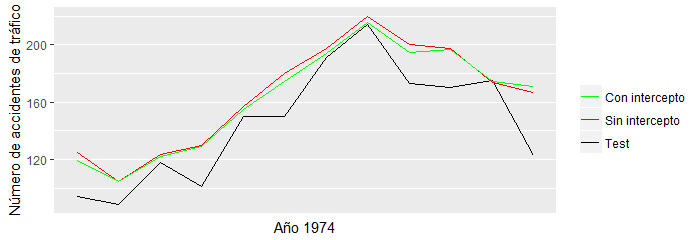
\includegraphics[scale = 0.7]{Images/Modelizacion/320.png}}
    \caption{Comparación de las predicciones del SARIMA$(1,0,1)(2,1,1)_{12}$ con y sin intercepto}
    \label{comp_sarimas}
\end{figure}

Existe un método realmente útil en esta librería encargado de seleccionar automáticamente el modelo, conocido como $\verb!auto.arima()!$. Se basa en un algoritmo que mediante la combinación del test de raíz unitaria, la optimización de los criterios de información y de la función de verosimilitud es capaz de seleccionar el modelo óptimo entre varios posibles. Los pasos que este algoritmo lleva a cabo son los siguientes:
\begin{enumerate*}
  \item Utiliza el test de la raíz unitaria de KPSS para determinar el número de diferencias necesarias, $d$, para lograr estacionariedad.
  \item A través del test OCSB de raíces unitarias estacionales determina el número necesario de diferencias $D$.
  \item Se selecciona $p$, $q$, $P$ y $Q$ de entre unos modelos iniciales de forma que se minimice el AICc, que no es más que una variación del AIC para muestras pequeñas.
  \item Se va variando progresivamente el orden y la presencia del intercepto del modelo seleccionado. Si el nuevo modelo tiene un AICc más bajo se toma este como referencia, en caso contrario se sigue con el anterior.
  \item Este último paso se repite hasta que no es posible encontrar otro modelo con un AICc más bajo.
  \item Ofrece como salida el último modelo seleccionado que, dado el funcionamiento del algoritmo, es el que minimiza el AICc.
\end{enumerate*}
\newpage
El proceso de selección se puede personalizar gracias a la sintaxis del método:
\begin{Verbatim}[fontsize=\footnotesize]
auto.arima(y, d = NA, D = NA, max.p = 5, max.q = 5, max.P = 2, max.Q = 2, max.d = 2,
           max.D = 1, ic = ("aicc", "aic", "bic"), test = c("kpss", "adf", "pp"),
           seasonal.test = c("ocsb", "ch"),...)
\end{Verbatim}

A través de $\verb!y!$ se introduce la serie a modelizar y en $\verb!d!$ y $\verb!D!$ se puede introducir las diferencias a realizar en cada parte de la serie, en caso de dejar estos argumentos por defecto lo decidirá el propio método gracias a varios test de raíz unitaria. A través de $\verb!max.d!$ y $\verb!max.D!$ se puede acotar superiormente las diferencias sobre las que buscar el modelo óptimo. Esto último también se puede aplicar a los parámetros a través de $\verb!max.p!$, $\verb!max.q!$, $\verb!max.P!$ y $\verb!max.Q!$. Se puede seleccionar el test a usar para seleccionar $d$ y $D$ gracias a los argumentos $\verb!test!$ y $\verb!seasonal.test!$. A través de $\verb!ic!$ podemos decidir sobre qué criterio se va a realizar la búsqueda del modelo óptimo.

Si aplicamos este método a nuestra serie $\verb!acc.train!$ especificando únicamente que utilice el test aumentado de la raíz unitaria de Dickey-Fuller para seleccionar $d$ obtenemos un SARIMA$(1,0,0)(1,0,0)_{12}$. Este modelo tiene un AIC de 1514.47, más alto que los dos anteriores y además hay correlaciones entre sus residuos. A pesar de esto el MAE del conjunto de test es de 14.86938, el mejor hasta ahora de todos los modelos  ARIMA ajustados.

El modelo que nos ofrece $\verb!auto.arima()!$ depende principalmente del algoritmo de búsqueda. Con ligeras variaciones en algunos de sus argumentos es posible obtener resultados completamente distintos. Por defecto esta búsqueda está configurada para tener un coste computacional bajo, sin embargo es posible forzar al algoritmo a que haga una búsqueda más exhaustiva pasando $\verb!stepwise!$ y $\verb!approximation!$ como $\verb!FALSE!$. Estos argumentos controlan el número de modelos sobre los que se realiza la búsqueda y la exactitud de los criterios usados. El argumento $\verb!max.order!$ fija el orden máximo del modelo de acuerdo a $p + q + P + Q$.

Hemos realizado esta búsqueda para nuestra serie fijando el $\verb!max.order!$ en 7. El modelo que nos ofrece es un SARIMA$(2,0,0)(2,0,0)_{12}$. En este caso el AIC es 1499.24 y el MAE de 14.96979. En el modelo anterior estamos realizando una buena predicción a pesar de tener un AIC superior al resto de modelos. En la Figura \ref{sarima_test} se aprecia como este modelo consigue detectar muy bien las fluctuaciones estacionales del conjunto de \textit{test}.
\begin{figure}
    \centering
    \centerline{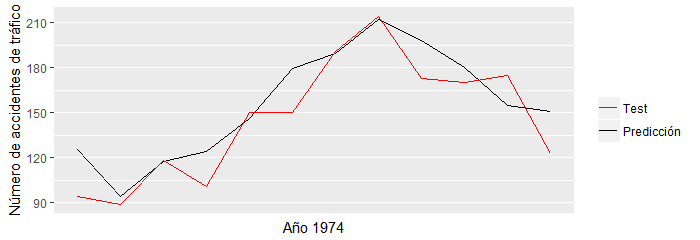
\includegraphics[scale = 0.7]{Images/Modelizacion/321.png}}
    \caption{Comparación de las predicciones del SARIMA$(2,0,0)(2,0,0)_{12}$ con el \textit{test}}
    \label{sarima_test}
\end{figure}

En la Tabla \ref{comp_2} se pueden ver las medidas de ajuste de distintos modelos. Se puede apreciar como el modelo con los mejores criterios de información es el SARIMA$(1,0,1)(2,1,1)_{12}$ con intercepto, además de que es el único con unos residuos puramente aleatorios. Sin embargo no es el que mejor predice ya que el mejor MAE le posee el SARIMA$(1,0,0)(1,0,0)_{12}$. Realmente no podemos decir que hay un modelo que destaque sobre los demás sino que algunos son mejores que otros en ciertos aspectos. Si queremos dar preponderancia al ajuste deberíamos fijarnos más en los criterios de información y en la aleatoriedad de los residuos mientras que si lo que buscamos son predicciones a corto-medio plazo deberíamos tener en cuenta medidas como el MAE. Al fin y al cabo la elección del modelo óptimo queda al criterio del usuario.
\begin{table}[]
\centering
\label{my-label}
\begin{tabular}{|l|c|c|c|c|c|}
\hline
\multicolumn{1}{|c|}{}                & AIC              & AICc             & BIC & MAE & Ljung Box \\ \hline
$(0,1,0)(0,0,2)_{12}$               & 1550.38          & 1550.53          & 1559.73                  & 22.19949                 & $\sim 0$                                   \\ \hline
$(1,0,1)(2,1,1)_{12 \thinspace sin \thinspace int}$ & 1367.68          & 1368.25          & 1385.98                  & 19.22651                 & 0.04321                                  \\ \hline
$(1,0,1)(2,1,1)_{12 \thinspace con \thinspace int}$ & \textbf{1359.82} & \textbf{1360.58} & \textbf{1381.17}         & 17.09992                 & \textbf{0.2748}                          \\ \hline
$(1,0,0)(1,0,0)_{12}$               & 1514.22          & 1514.47          & 1526.72                  & \textbf{14.86938}        & 0.00085                                   \\ \hline
$(2,0,0)(2,0,0)_{12}$                & 1499.24          & 1499.77          & 1517.99                  & \textbf{14.96979}        & 0.002708                                  \\ \hline
$(1,1,4)(2,0,0)_{12}$               & 1485.29          & 1486.2           & 1510.24                  & 23.44705                 & 0.01353                                  \\ \hline
\end{tabular}
\caption{Comparación de los distintos SARIMA ajustados}
\label{comp_2}
\end{table}

\section{TSeries Package}
La librería $\verb!tseries!$ contiene métodos tanto de preprocesado como de modelización de serie temporales, además de varios test estadísticos orientados a series temporales. Aunque muchos de sus métodos están orientados al análisis de series financieras es posible aplicarlos, tras las transformaciones oportunas, a series con una temática más general \cite{tseries}.

Vamos a cargar los datos en el formato $\verb!zoo!$ y $\verb!ts!$ aunque básicamente utilizaremos este último dado que nos apoyaremos en algunos métodos de las librerías $\verb!stats!$ y $\verb!forecast!$ (se puede ver el código en el Anexo VII).

\subsection{Preprocesado}
Comenzaremos desestacionalizando nuestra serie a fin de poder aplicar más adelante un modelo ARMA. Para ello vamos a estimar las distintas componentes a través del método $\verb!decompose()!$ y con $\verb!seasadj()!$ de $\verb!forecast!$ vamos a eliminar la componente estacional. En esta ocasión vamos a trabajar bajo el supuesto de aditividad y además vamos a realizar la división en \textit{training} y \textit{test} después de la desestacionalización y no antes. El resultado se muestra en la Figura \ref{acc_deses}.
\begin{figure}
    \centering
    \centerline{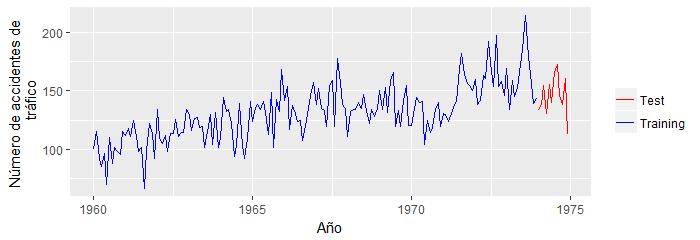
\includegraphics[scale = 0.7]{Images/Modelizacion/322.png}}
    \caption{Serie \PVerb{accidentes} desestacionalizada con \PVerb{seasadj()}}
    \label{acc_deses}
\end{figure}

Debido a la naturaleza del modelo a aplicar debemos trabajar bajo el supuesto de estacionariedad. Para ello aplicaremos tres test distintos implementados en esta librería:
\begin{itemize*}
  \item[$\bullet$] \textbf{Test aumentado de Dickey-Fuller}: Implementado por $\verb!adf.test()!$, nos permite contrastar tanto el supuesto de estacionariedad (raíz unitaria) como de explosividad (raíz fuera del círculo unidad). Para elegir entre un ajuste u otro debemos modificar el argumento $\verb!alternative!$ ($\verb!"stationary"!$ o $\verb!"explosive"!$).
  \item[$\bullet$] \textbf{Test de Philipps-Perron}: El método que lo implementa es $\verb!pp.test()!$ y funciona de la misma manera que $\verb!adf.test()!$. Este test se deriva del de Dickey-Fuller solo que utiliza técnicas no paramétricas para aproximar la distribución del estadístico.
  \item[$\bullet$] \textbf{Test de KPSS}: Contrasta la hipótesis nula de que la serie es estacionaria en tendencia frente a la presencia de raíz unitaria. Se implementa a través de $\verb!kpss.test()!$. Para trabajar bajo la tendencia aquí tratada se debe introducir el argumento $\verb!null!$ como $\verb!"Trend"!$.
\end{itemize*}

En los test de Dickey-Fuller y Phillipps-Perron estamos obteniendo unos p-valores para los contrastes de estacionariedad y explosividad de 0.01 y 0.99, respectivamente.  Esto significa que parece haber indicios de estacionariedad en nuestra serie ya que hemos rechazado la hipótesis nula de raíz unitaria y no hemos podido rechazar la de no explosividad. El p-valor para el test de KPSS es de 0.05506 por lo que no podemos rechazar la hipótesis nula de estacionariedad en tendencia, sin embargo si observamos la serie apreciamos que sí que parece haber tendencia no constante por lo que vamos a diferenciar la serie para eliminarla. El resultado se muestra en la Figura \ref{acc_deses_diff}.
\begin{figure}
    \centering
    \centerline{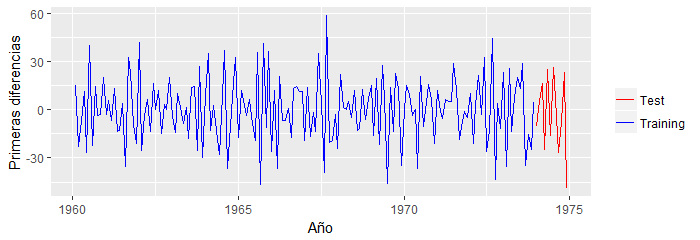
\includegraphics[scale = 0.7]{Images/Modelizacion/323.png}}
    \caption{Serie \PVerb{accidentes} desestacionalizada y diferenciada}
    \label{acc_deses_diff}
\end{figure}

Tras esta transformación obtenemos los mismos resultados en los test de Dickey-Fuller y Phillips-Perron, sin embargo ahora nos sale un p-valor para el test de KPSS de 0.1, lo que significa que no podemos rechazar la hipótesis de estacionariedad en tendencia. Trabajaremos con esta serie ya que parece haber fuertes evidencias estadísticas de estacionariedad.

Existen test encargados de contrastar la linealidad de la tendencia de series temporales a través de métodos basados en redes neuronales. Esta librería incorpora dos métodos capaces de implementar los test de no linealidad: Terasvirta y White. Aunque ambos tests funcionan de forma similar, el de White es más restrictivo ya que consigue diferenciar en el contraste la no linealidad arbitraria. Los respectivos métodos son $\verb!terasvirta.test()!$ y $\verb!white.test()!$ y trabajan bajo la hipótesis nula de linealidad en media. Para el tipo de serie que manejamos basta con dejar los argumentos por defecto. Obtenemos un p-valor de 0.8989 en el test de Terasvirta y de 0.7783 en el de White, por lo que nuestra serie parece seguir una tendencia lineal (algo lógico ya que hemos dejado la tendencia constante al diferenciar).

Existe un método en esta librería conocido como $\verb!maxdrawdown()!$ que se encarga de extraer la mayor disminución de la serie, es decir, nos devuelve el periodo con mayor diferencia entre el valor inicial y el final. En nuestro caso ese periodo se corresponde al comprendido entre septiembre de 1967 y julio de 1969, con una diferencia de 104.3482 unidades. Estas unidades ya no se pueden interpretar como accidentes ya que hemos realizado varias transformaciones a la serie.

\subsection{Técnicas de remuestreo}
Gracias al desarrollo de la computación se han popularizado las técnicas de remuestreo, una de las más conocidas es el \textit{bootstrap} \cite{efron_bootstrap_1979}. En ocasiones queremos estimar un parámetro poblacional y para ello contamos únicamente con una muestra. Con esta técnica extraemos submuestras de esa muestra a través de un muestreo aleatorio con reposición y de estas submuestras se obtiene el estadístico deseado. Esto se repite un gran número de veces pudiendo así construir una aproximación de la distribución del estadístico a través de las submuestras.

Esta técnica se puede aplicar a series temporales, solo que necesitamos hacer algunas modificaciones. No podemos aplicar un muestreo aleatorio ya que perderíamos la característica que define a las series temporales, la correlación temporal. En este caso se utiliza una variación del \textit{bootstrap} original conocido como \textit{bootstrap} por bloques. El método encargado de implementar esto es $\verb!tsbootstrap()!$ y su sintaxis es la siguiente:
\begin{Verbatim}[fontsize=\footnotesize]
tsbootstrap(x, nb = 1, statistic = NULL, m = 1, b = NULL,
            type = c("stationary","block"), ...)
\end{Verbatim}

A través de $\verb!x!$ se introduce la serie y a partir de $\verb!nb!$ el número de series a generar (submuestras). El argumento $\verb!type!$ define el tipo de \textit{bootstrap} a aplicar, las opciones disponibles son las siguientes:
\begin{itemize*}
  \item[$\bullet$] \textbf{Por bloques} (\PVerb{"block"}): La serie se divide en  $n-b+1$ bloques de longitud $b$ de forma que el primer bloque contendrá las observaciones $Y_1,...,Y_b$, el segundo las observaciones $Y_2,...,Y_{b+1}$, etc… Sobre estos bloques se hace un muestreo aleatorio con remplazamiento seleccionando $n/b$ bloques y se combinan sin alterar su orden en la serie original de forma que obtenemos una nueva serie capaz de replicar la autocorrelación temporal.
  \item[$\bullet$] \textbf{Estacionario} (\PVerb{"stationary"}): El procedimiento es el mismo solo que en este caso $b$ no es fijo sino que varía aleatoriamente. Con esta pequeña modificación nos aseguramos la estacionariedad de la nueva serie.
\end{itemize*}

El argumento $\verb!b!$ fija la longitud de los bloques si trabajamos bajo el tipo $\verb!"block"!$, en caso de hacerlo bajo $\verb!"stationary"!$ fija la media de la longitud de los bloques, es decir, la media de los valores aleatorios generados. Se recomienda que $b$ aumente con $n$, por ello por defecto el valor de $b$ es proporcional a $n^3$. Si el argumento $\verb!statistic!$ se deja por defecto el método nos devolverá la serie remuestrada, en caso de que se introduzca alguna función como $\verb!mean()!$ o $\verb!sd()!$, nos devolverá el estadístico aplicado a la serie original y la estimación del sesgo y del error estándar a través de las series generadas por el \textit{bootstrap}.

El argumento $\verb!m!$ introduce una pequeña variación en el \textit{bootstrap}. Por defecto vale 1, esto mantiene el proceso como se ha descrito pero si $\PVerb{m} > 1$ divide la serie original en bloques de longitud $m$ y aplica el \textit{bootstrap} individualmente a esos bloques, en vez de a la serie en su totalidad. Como en este caso la serie original se ha divido, el estadístico aplicado a la serie original varía. En la Figura \ref{bootstrap} se muestran las series generadas por un \textit{bootstrap} por bloques y estacionario con los argumentos $\verb!m!$ y $\verb!b!$ por defecto.

\begin{figure}
    \centering
    \centerline{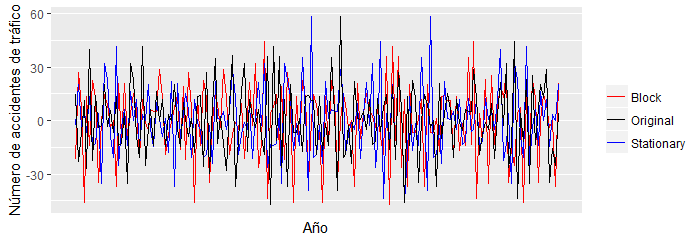
\includegraphics[scale = 0.7]{Images/Modelizacion/32413242.png}}
    \caption{El método \PVerb{tsbootstrap()} aplicado a la serie \PVerb{acc.train.dif.adj}}
    \label{bootstrap}
\end{figure}

Vamos a definir una función $\verb!initial.acf()!$ que nos devuelva los siete primeros valores del correlograma de la función de autocorrelación (excluyendo el primero). Tras esto vamos a hacer un \textit{bootstrap} estacionario sobre nuestra serie para intentar estimar estas correlaciones a través de 500 submuestras de la serie. La salida resultante es la siguiente:
\vspace{1cm}
\begin{Verbatim}[fontsize=\footnotesize]
          Call:
          tsbootstrap(x = acc.train.dif.adj, nb = 500, statistic =
          initial.acf, type = "stationary")

          Resampled Statistic(s):
             original      bias std. error
          t1 -0.46105  0.032406    0.04939
          t2  0.05999 -0.021088    0.08265
          t3 -0.00991  0.010304    0.08036
          t4 -0.11464  0.016317    0.08634
          t5  0.07060  0.001765    0.08768
          t6 -0.01765  0.009458    0.07539
          t7 -0.08207  0.011581    0.07784
\end{Verbatim}

En primer lugar nos muestra las características del \textit{bootstrap} utilizado. Después vemos los valores de los estadísticos (en este caso las autocorrelaciones) en la muestra acompañados del sesgo y el error estándar obtenidos gracias al \textit{bootstrap}.

Un método similar incluido en esta librería es $\verb!surrogate()!$. Las series temporales no son más que funciones periódicas en el tiempo por lo que en ocasiones se utilizan transformadas de Fourier para describirlas. Este método recurre a este tipo de técnicas para generar subseries con una estructura similar a la original. Su sintaxis es la siguiente:
\begin{Verbatim}[fontsize=\footnotesize]
surrogate(x, ns = 1, fft = FALSE, amplitude = FALSE, statistic = NULL, ...)
\end{Verbatim}

A través de $\verb!x!$ se introduce la serie y en $\verb!ns!$ se indica el número de series a generar. Si los argumentos $\verb!fft!$ y $\verb!amplitude!$ se dejan en $\verb!FALSE!$ lo único que hace es generar las nuevas series a partir de permutaciones de la original perdiendo así toda la correlación temporal. En este tipo de técnicas el espectro recoge la distribución de amplitudes que definen al proceso modelado, el argumento $\verb!fft!$ consigue generar una nueva serie basada en el espectro de la original introduciendo cierta aleatorización en la fase de los coeficientes de Fourier. El argumento $\verb!amplitude!$ consigue mantener en las nuevas series las amplitudes de la original. En la Figura \ref{surrogate} se muestra la serie original junto a una generada a partir de este método con los argumentos $\verb!fft!$ y $\verb!amplitude!$ como $\verb!TRUE!$.
\begin{figure}
    \centering
    \centerline{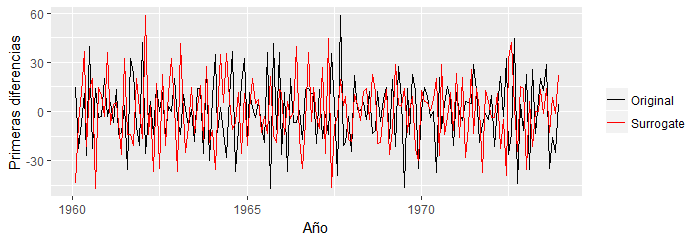
\includegraphics[scale = 0.7]{Images/Modelizacion/325.png}}
    \caption{El método \PVerb{surrogate()} aplicado a la serie \PVerb{acc.train.dif.adj}}
    \label{surrogate}
\end{figure}

\subsection{Modelos ARMA}
Una vez preparada la serie vamos a ajustarle un modelo ARMA. Como esta librería no incluye ningún método para la detección automática del orden de los parámetros vamos a estudiar sus correlogramas a partir de los métodos $\verb!Acf()!$ y $\verb!Pacf()!$ de la librería $\verb!forecast!$. Los resultados se muestran en la Figura \ref{a_p}. En el ACF se puede apreciar como únicamente la primera autocorrelación es significativa por lo que vamos a suponer $q = 1$ para la parte de medias móviles. En el PACF vemos que tanto la primera como la segunda autocorrelación son significativas, considerando parsimoniosidad vamos a suponer $p = 1$ para la parte autorregresiva.
\begin{figure} [t]
\begin{subfigure}{.5\textwidth}
  \centering
  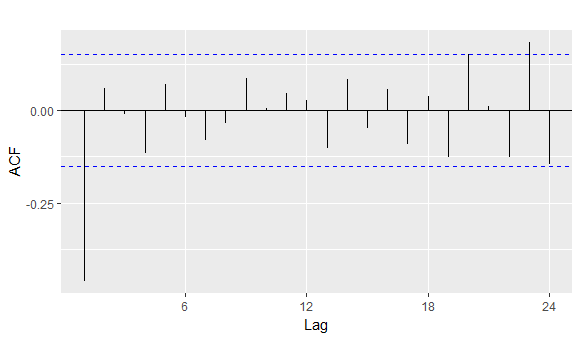
\includegraphics[width=.8\linewidth]{Images/Modelizacion/3261.png}
  \caption{ACF}
  \label{fig:sfig1}
\end{subfigure}
\begin{subfigure}{.5\textwidth}
  \centering
  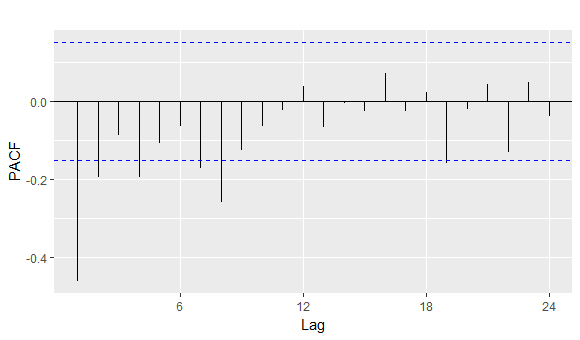
\includegraphics[width=.8\linewidth]{Images/Modelizacion/3262.png}
  \caption{PACF}
  \label{fig:sfig2}
\end{subfigure}
\caption{Correlogramas para la serie \PVerb{acc.train.dif.adj}}
\label{a_p}
\end{figure}

El método encargado de implementar los modelos ARMA en esta librería es $\verb!arma()!$. Su sintaxis es similar al $\verb!Arima()!$ de $\verb!forecast!$ ya que ambos se sustentan en el $\verb!arima()!$ de $\verb!stats!$:
\begin{Verbatim}[fontsize=\footnotesize]
arma(x, order = c(1, 1), lag = NULL, coef = NULL,
     include.intercept = TRUE, qr.tol = 1e-07, ...)
\end{Verbatim}

En $\verb!x!$ se introduce la serie a modelizar y tanto en $\verb!order!$ como en $\verb!lag!$ se puede introducir los órdenes de la parte autorregresiva y de la medias móviles. Si se introduce ambos argumentos se da prioridad a lo especificado en $\verb!order!$. A través del argumento $\verb!coef!$ se puede introducir una inicialización personalizada de los coeficientes para el proceso de estimación, recomiendo dejarlo por defecto. Con $\verb!include.intercept!$ incluimos el intercepto en el modelo y con $\verb!qr.tol!$ definimos la tolerancia que se utiliza para calcular el error estándar de los coeficientes. Para ajustar un ARMA$(1,1)$ sin intercepto a nuestra serie debemos escribir el siguiente código:
\begin{Verbatim}[fontsize=\footnotesize, numbers = left]
model.1 <- arma(acc.train.dif.adj, order = c(1,1), include.intercept = FALSE)
summary(model)
\end{Verbatim}

Al trabajar bajo la serie original diferenciada lo que realmente estamos ajustando es un ARIMA$(1,1,1)$. Estamos obteniendo un AIC de 1419.3 que aunque no es el mejor supera al de otros modelos ajustados con $\verb!forecast!$. Si graficamos el correlograma de los residuos vemos que ninguna autocorrelación es significativa por lo que parece que el modelo recoge todos los patrones de la serie. A través del método $\verb!jarque.bera.test()!$ incluido en este librería vamos a contrastar la normalidad de los residuos con el test de Jarque Bera. Obtenemos un p-valor de 0.5357 por lo que podemos afirmar que los residuos siguen una distribución normal, confirmando lo visto en el correlograma.  Otro método bastante útil para estudiar los residuos es $\verb!bds.test()!$. Este método implementa el test no paramétrico de BDS que contrasta la hipótesis nula de que los datos son independientes e idénticamente distribuidos (i.i.d). Su sintaxis es la siguiente:
\begin{Verbatim}[fontsize=\footnotesize, numbers = left]
bds.test(x, m = 3, eps = seq(0.5 * sd(x), 2 * sd(x),
                             length = 4),...)
\end{Verbatim}

Para ver cómo funciona este test definamos las siguientes probabilidades:
\begin{equation}
    P_1 = P(\lvert Y_i - Y_j \lvert < \epsilon)\quad \text{con} \quad i \neq j, \quad i,j \in T
\end{equation}
\begin{equation}
    P_m = P(\lvert Y_i - Y_j \lvert < \epsilon, \lvert Y_{i-1} - Y_{j-1} \lvert < \epsilon,...,\lvert Y_{i-m} - Y_{j-m} \lvert < \epsilon)
\end{equation}

Lo que estamos calculando en (68) es la probabilidad de que dos observaciones de nuestra serie no disten más de $\epsilon$, sin embargo en (69) estamos calculando la probabilidad de que tanto esas dos observaciones como sus $m$ anteriores no disten entre sí más de $\epsilon$. Si la serie $Y_t$ es independiente e idénticamente distribuida (i.i.d) por definición se tiene que:
\begin{equation}
    {P_1}^m = P_m
\end{equation}

Por lo tanto el test BSD contrasta lo siguiente:
\begin{align}
    H_0 &: {P_1}^m = P_m \rightarrow i.i.d\\
    H_1 &: {P_1}^m \neq P_m \rightarrow no \: i.i.d
\end{align}

El argumento $\verb!m!$ fija hasta dónde llega $m$ partiendo de 2 (por defecto es 3 por lo que $\verb!m!$ tomará los valores 2 y 3) y $\verb!eps!$ los valores de $\epsilon$. Como salida obtendremos $m \times \epsilon$ p-valores correspondientes a los resultados del test para las distintas combinaciones. Los p-valores para nuestros residuos dejando los argumentos por defecto son los siguientes:
\begin{Verbatim}[fontsize=\footnotesize]
         p-value =
               [ 8.3335 ] [ 16.667 ] [ 25.0004 ] [ 33.3339 ]
         [ 2 ]     0.4068     0.4443      0.4235      0.2465
         [ 3 ]     0.4032     0.9104      0.6961      0.4041
\end{Verbatim}

Obtenemos para todas las combinaciones p-valores mayores de 0.05 por lo que podemos afirmar que los residuos son i.i.d.

Hemos ajustado también un ARIMA$(2,1,1)$ para ver si mejora el modelo anterior (hemos tenido en cuenta la segunda autocorrelación de la Figura \ref{a_p}). Obtenemos un AIC de 1414.81, algo más bajo que el anterior. El test de Jarque Bera nos arroja un p-valor de 0.7782 y todos los p-valores del test BSD son mayores a 0.05. Todos estos indicios nos sugieren que este modelo también parece recoger todos los patrones contenidos en los datos ya que los residuos parecen ser ruido. En la Figura \ref{fit_arma} se muestra el ajuste de este último modelo.
\begin{figure}
    \centering
    \centerline{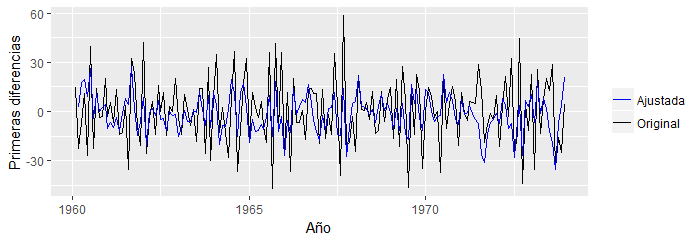
\includegraphics[scale = 0.7]{Images/Modelizacion/3272.png}}
    \caption{Ajuste del modelo ARIMA$(2,1,1)$ implementado con \PVerb{arma()}}
    \label{fit_arma}
\end{figure}

Esta librería no incluye ningún método para predecir a partir de los objetos generados por $\verb!arma()!$ por lo que no nos ha sido posible comparar ambos modelos de acuerdo a su poder predictivo.

\section{FitARMA Package}
Hasta ahora hemos visto librerías que incluían métodos generales para el análisis de series temporales, sin embargo existen otras más especializadas en ciertos aspectos de estas. La librería $\verb!FitARMA!$ únicamente incluye métodos orientados a la implementación de modelos ARIMA \cite{fitarma}.

Al no incluir modelos capaces de tratar la componente estacional vamos a desestacionalizar la serie de la misma manera en que lo hemos hecho para $\verb!tseries!$. Como la tendencia sigue dependiendo del tiempo también la vamos a diferenciar. El resultado son las series $\verb!acc.train.dif.adj!$ y $\verb!acc.test.dif.adj!$ que se mostraron en la Figura \ref{acc_deses_diff} (el código se encuentra en el Anexo VIII).

El método principal de esta librería es $\verb!FitARMA()!$ encargado de implementar los modelos ARIMA. Se caracteriza por el algoritmo de estimación que utiliza para ajustar el modelo a nuestros datos. Este algoritmo se sustenta en la estimación por máxima verosimilitud solo que consigue reducir los cálculos necesarios a través de una aproximación de esta \cite{fitarma-algoritmo}.

La sintaxis de este método es la siguiente:
\begin{Verbatim}[fontsize=\footnotesize]
FitARMA(z, order = c(0, 0, 0), demean = TRUE, MeanMLEQ = FALSE,
        pApprox = 30, MaxLag = 30)
\end{Verbatim}

A través de $\verb!z!$ introducimos la serie a modelizar y en $\verb!order!$ los valores de los parámetros $p$, $d$ y $q$ del modelo a ajustar. Si mantenemos $\verb!demean!$ como $\verb!TRUE!$ incluiremos el intercepto en el modelo. Si además queremos estimar el intercepto a través de este algoritmo debemos pasar el argumento $\verb!MeanMLEQ!$ como $\verb!TRUE!$. El algoritmo consigue aproximar la función de máximo verosimilitud del ARMA a través de un AR de un orden bastante superior, el argumento $\verb!pApprox!$ es el que indica al algoritmo el orden de este AR. Como este método implementa internamente el test de Ljung-Box deberemos indicarle a través de $\verb!MaxLag!$ el número de rezagos que debe utilizar.

Comenzaremos ajustando un ARMA$(2,1)$ a la serie $\verb!acc.train.dif.adj!$ dejando el resto de los argumentos del método por defecto. Si hacemos $\verb!summary()!$ sobre el modelo obtenemos la siguiente salida:
\begin{Verbatim}[fontsize=\footnotesize]
ARIMA(2,0,1)
length of series = 167 ,  number of parameters = 4
loglikelihood = -465.75 ,  aic = 939.5 ,  bic =  952
\end{Verbatim}

Destacar el bajo valor del AIC en comparación con los modelos ajustados con otras librerías. En este caso el AIC solo es comparable entre modelos con $d = 0$, además de entre aquellos ajustados con este método. Con $\verb!coef()!$ podemos obtener información acerca de los coeficientes del modelo, la correspondiente salida se muestra a continuación:
\begin{Verbatim}[fontsize=\footnotesize]
                        MLE         sd   Z-ratio
          phi(1)   0.2259977 0.08360269  2.703235
          phi(2)   0.1443701 0.08246120  1.750764
          theta(1) 0.9477932 0.02999630 31.597007
          mu       0.2586612 7.97254543  0.032444
\end{Verbatim}

Nos muestra tanto el valor de los coeficientes como sus desviaciones estándar. Además nos muestra también el estadístico $Z$ para cada uno de los coeficientes. Estamos trabajando a un nivel de significación de 0.05 que le corresponde un valor crítico de 1.96 por lo que únicamente $\phi_1$ y $\theta_1$ son significativamente distintos de cero.

Aunque es posible obtener las autocorrelaciones de los residuos a través del \textit{subsetting} $\verb!$racf!$ vamos a seguir recurriendo al método $\verb!Acf()!$. En la Figura \ref{residuos} se puede apreciar como ninguna autocorrelación resulta significativa. Además el test de Ljung-Box implementado por el propio método nos ofrece p-valores superiores a 0.05 para todos los rezagos.
\begin{figure}
    \centering
    \centerline{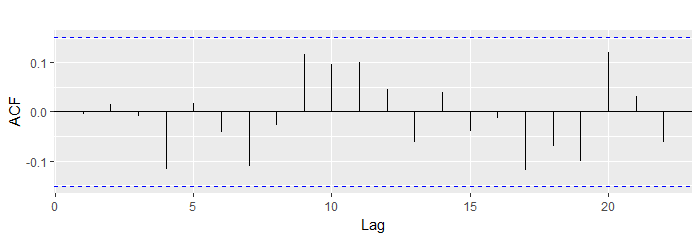
\includegraphics[scale = 0.7]{Images/Modelizacion/328.png}}
    \caption{Correlograma para los residuos del ARMA$(2,1)$}
    \label{residuos}
\end{figure}

El modelo anterior ha trabajado con $\PVerb{MeanMLEQ} = \PVerb{FALSE}$, vamos a pasarlo como $\verb!TRUE!$ para ver si afecta notablemente al ajuste. A continuación se muestra el código:
\begin{Verbatim}[fontsize=\footnotesize, numbers = left]
model.2 <- FitARMA(acc.train.dif.adj, order = c(2,0,1), MeanMLEQ = TRUE)
summary(model.2)
\end{Verbatim}

En este caso nos está devolviendo un AIC de 938.5 que es ligeramente menor al del modelo anterior, sin embargo la significatividad de los parámetros sigue siendo la misma. Los residuos de los modelos siguen mostrando suficientes evidencias estadísticas como para poder afirmar que son ruido. Aunque la diferencia en los AIC de los modelos es mínima supone una razón suficiente para hacernos decantar por este segundo modelo, es decir, por la estimación del intercepto a través del algoritmo de la librería. En la Figura \ref{arma_fitarma} se muestra el ajuste de este modelo a los datos.
\begin{figure}
    \centering
    \centerline{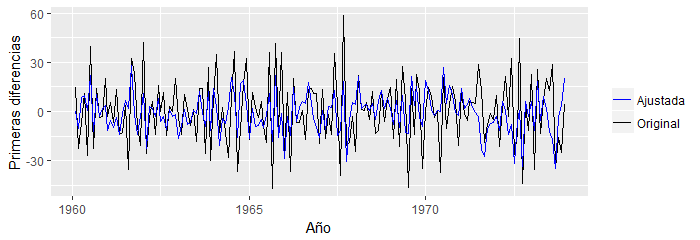
\includegraphics[scale = 0.7]{Images/Modelizacion/329.png}}
    \caption{Ajuste del modelo ARMA$(2,1)$ implementado con \PVerb{FitARMA()}}
    \label{arma_fitarma}
\end{figure}

Para intentar mejorar aún más este modelo vamos a intentar obtener el valor óptimo de $\verb!pApprox!$. Realizaremos ajustes para distintos valores de este parámetro y estudiaremos la verosimilitud para intentar localizar el óptimo. Probaremos a ajustar los distintos modelos de acuerdo a los valores 10, 20, 30, 40, 50, 60, 70 y 80 para $\verb!pApprox!$. En la Figura \ref{logaritmo} se muestra este estudio. Se puede observar que la verosimilitud desciende hasta alcanzar su valor mínimo con $\PVerb{pApprox} = 20$, sin embargo después parece incrementar a medida que se aumenta el valor del argumento. Lo que este estudio parece decirnos es que los valores de $\verb!pApprox!$ que maximizan la verosimilitud son aquellos más altos. Sabiendo esto vamos a ajustar el mismo modelo que antes solo que ahora vamos a pasar $\verb!pApprox!$ como 80, su $\verb!summary()!$ se muestra a continuación:
\begin{Verbatim}[fontsize=\footnotesize]
ARIMA(2,0,1)  With mean MLE.
length of series = 167 ,  number of parameters = 4
loglikelihood = -464.52 ,  aic = 937 ,  bic =  949.5
\end{Verbatim}

\begin{figure}
    \centering
    \centerline{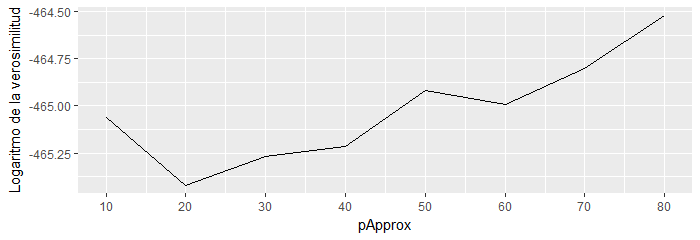
\includegraphics[scale = 0.7]{Images/Modelizacion/330.png}}
    \caption{Evolución del logaritmo de la verosimilitud respecto a \PVerb{pApprox}}
    \label{logaritmo}
\end{figure}

En este caso estamos obteniendo un AIC de 937, el más bajo hasta el momento. Este resultado parece mostrar que el argumento $\verb!pApprox!$ juega internamente un papel importante en el método.

A continuación vamos a comparar la eficiencia de este método respecto a sus equivalentes en las librerías $\verb!forecast!$ y $\verb!tseries!$ ($\verb!Arima()!$ y $\verb!arma()!$). Para ello vamos a estudiar sus tiempos con el método $\verb!system.time()!$. Ajustaremos a la serie $\verb!acc.train.dif.adj!$ un modelo ARMA$(2,1)$ a través de los tres métodos distintos y guardaremos el tiempo interno que tarda el ordenador en realizar cada uno de estos ajustes. Repetiremos este proceso 50 veces para poder apreciar cómo se comportan cada uno de los tres métodos.

En la Figura \ref{tiempos_modelos} se muestran los resultados de esta simulación. En el eje de las abscisas se muestra el número de simulación mientras que en el de las ordenadas el tiempo empleado por el ordenador para llevar a cabo el ajuste. Lo que más llama la atención es la gran diferencia de tiempos entre el método de $\verb!FitARMA!$ y los de $\verb!forecast!$ y $\verb!tseries!$. El algoritmo implementado en $\verb!FitARMA!$ ofrece rapidez para cantidades grandes de datos, sin embargo parece que para cantidades pequeñas se estanca, tardando casi tres veces más que el resto de métodos. Además parece mostrar un comportamiento muy errático, mostrando grandes variaciones en los tiempos cuando realmente su comportamiento debería mantenerse más o menos constante (la presencia de estas variaciones se debe principalmente a los procesos llevados a cabo por el ordenador en segundo plano). Los métodos implementados en $\verb!forecast!$ y $\verb!tseries!$ parecen comportarse de una forma más estable.
\begin{figure}
    \centering
    \centerline{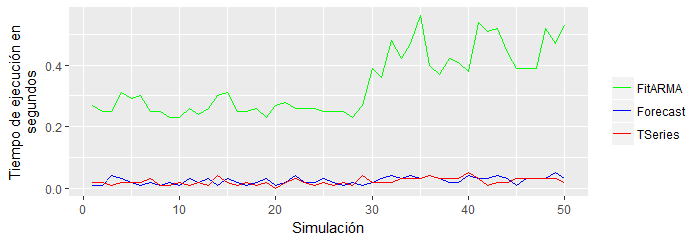
\includegraphics[scale = 0.7]{Images/Modelizacion/331.png}}
    \caption{Comparación de tiempos para los métodos de ajuste de modelos ARMA}
    \label{tiempos_modelos}
\end{figure}

\section{Opera Package}
Hasta ahora hemos utilizado modelos de distintas librerías para realizar predicciones sobre nuestra serie temporal. Lo que buscamos es optimizar el poder predictivo del modelo por lo que normalmente seleccionaremos aquel que nos ofrezca las predicciones más acertadas. Pero existen otros enfoques con los que podemos obtener mejores resultados.

Por la propia naturaleza de los distintos modelos tenemos que unos recogerán comportamientos indetectables por otros. Bajo estos supuestos tiene sentido combinar las predicciones de los distintos modelos a fin de intentar recoger toda la información posible. Una de las librerías encargada de implementar este tipo de técnicas es $\verb!opera!$ \cite{opera}. Se puede estudiar el código utilizado en este apartado en el Anexo IX.

Consideremos una serie de la forma $Y_1, Y_2,...,Y_t$. Hemos ajustado $K$ modelos cada uno de los cuales nos ofrece una predicción distinta para el tiempo $t+h$, a estas predicciones las denotaremos como $x_{k,t+h}$. Después calcularemos $\widehat{Y}_{t+h}$ combinando todas estas predicciones ponderando de acuerdo a su rendimiento, es decir:
\begin{equation}
    \widehat{Y}_{t+h} = \sum_{k = 1}^{K} p_{k,t+h} \enskip  x_{k,t+h}
\end{equation}

\noindent donde las ponderaciones $p_{k,t+h}$ se fijan de acuerdo al poder predictivo de los distintos modelos. Una de las principales características de este tipo de técnicas es que pueden implementarse en línea, es decir, pueden ir ajustando las ponderaciones a medida que se introducen nuevos valores del \textit{test}. Para entenderlo mejor a continuación se muestra el proceso que suelen seguir estas últimas:
\begin{enumerate*}
  \item Inicializamos las ponderaciones $p_{k,t+1}$ uniformemente.
  \item Calculamos las predicciones para el tiempo $t+1$ de los distintos K modelos ($x_{k,t+1}$).
  \item Calculamos $\widehat{Y}_{t+1}$ a partir de la suma ponderada de estas $K$ predicciones.
  \item Introducimos el valor real de la serie y ajustamos las ponderaciones de acuerdo a la función de pérdida definida.
  \item Estas ponderaciones ajustadas se denotan como $p_{k,t+2}$ y se utilizan para calcular $\widehat{Y}_{t+2}$.
  \item Se itera el proceso hasta que no tengamos más observaciones en nuestro conjunto de \textit{test}.
\end{enumerate*}

Este tipo de procesos son perfectos para modelos en los que la variable dependiente sigue una estructura temporal ya que este se puede ir actualizando a medida que tenemos nuevas observaciones de la serie.
\begin{figure}
    \centering
    \centerline{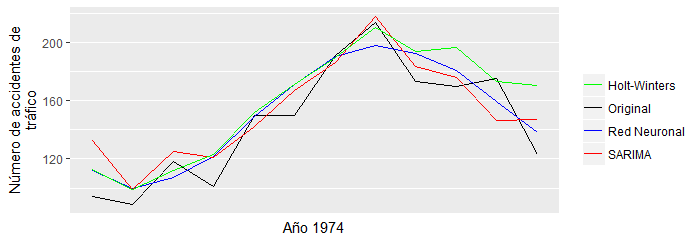
\includegraphics[scale = 0.7]{Images/Modelizacion/332.png}}
    \caption{Comparación del ajuste de los distintos modelos}
    \label{comp_entre_modelos}
\end{figure}

Vamos a combinar las predicciones a un año de tres modelos previamente ajustados: red neuronal, SARIMA$(1,0,0)(1,0,0)_{12}$ y triple suavizado de Holt-Winters. Sus respectivos MAE son de 13.27784, 14.86938 y 15.04762 y sus ajustes se muestran en la Figura \ref{comp_entre_modelos}. Para trabajar con los métodos de esta librería es necesario tener las predicciones de los tres modelos en un mismo objeto:
\begin{Verbatim}[fontsize=\footnotesize, numbers = left]
X <- cbind(red = pred.red$mean, sarima = pred.sarima$mean, hw = pred.hw$mean)
\end{Verbatim}

Es posible estudiar el error a nivel observacional gracias al método $\verb!loss()!$. Este método nos muestra el error cometido por cada uno de los tres modelos en cada observación del \textit{test}, su sintaxis es la siguiente:
\begin{Verbatim}[fontsize=\footnotesize]
loss(x, y, loss.type = "square")
\end{Verbatim}

A través de $\verb!x!$ se introducen las predicciones de los modelos, en $\verb!y!$ el conjunto de \textit{test} con el que se va a comparar y en $\verb!loss.type!$ el tipo de función de pérdida a utilizar.  Por defecto viene la cuadrática ($\verb!square!$) pero nosotros utilizaremos la absoluta ($\verb!absolute!$), que se corresponde con el MAE. En nuestro caso la salida resultante es la siguiente:
\begin{Verbatim}[fontsize=\footnotesize]
                          red    sarima        hw
          Jan 1974 18.0127432 38.527985 18.450649
          Feb 1974 10.9568480 10.320400  9.710105
          Mar 1974 11.0906385  7.150485  5.664850
          Apr 1974 20.4867823 19.718444 22.231049
          May 1974  0.6093056  7.863369  1.744073
          Jun 1974 21.3113668 17.094233 21.410794
          Jul 1974  0.7535920  4.476612  1.277397
          Aug 1974 15.9864688  3.778124  3.435301
          Sep 1974 19.4924576 10.727018 20.507963
          Oct 1974 10.5408218  6.081625 26.904985
          Nov 1974 15.2725507 28.796364  1.528908
          Dec 1974 14.7910821 23.897923 47.705347
\end{Verbatim}

Podemos apreciar como el MAE del SARIMA y el Holt-Winters parece mostrar un comportamiento irregular ya que intermensualmente varía mucho, sin embargo el MAE de la red neuronal parece mostrar un comportamiento más estable con variaciones más suaves.

\subsection{Combinaciones fuera de línea}
El método $\verb!oracle()!$ implementa una técnica para la combinación de predicciones no aplicable en línea ya que necesita desde un principio el conjunto de \textit{test} en su totalidad. Su sintaxis se muestra a continuación:
\begin{Verbatim}[fontsize=\footnotesize]
oracle(Y, experts, model = "convex", loss.type = "square",
       lambda = NULL, niter = NULL, ...)
\end{Verbatim}

En $\verb!Y!$ introducimos el conjunto de \textit{test} y en $\verb!experts!$ el objeto que contiene las predicciones realizadas por los tres modelos. A través de $\verb!model!$ especificaremos el tipo de combinación a utilizar, las principales opciones son las siguientes:
\begin{description}
  \item[$\bullet$ \PVerb{Expert}:]Selecciona las predicciones del modelo con mejor rendimiento.
  \item[$\bullet$ \PVerb{Convex}:]Selecciona la combinación convexa óptima para las distintas predicciones. Se cumple que para $\forall i \in K$:
  \begin{equation}
    p_{i,t+h} > 0
  \end{equation}
  \begin{equation}
    \sum_{i}^{} p_{i,t+h} = 1
  \end{equation}
  \item[$\bullet$ \PVerb{Linear}:]Selecciona la combinación lineal óptima para las distintas predicciones.
\end{description}

El argumento $\verb!loss.type!$ indica el tipo de función de pérdida a utilizar. El resto de argumentos ofrecen personalizaciones más complejas como la inclusión del parámetro de regularización para el caso lineal. Comenzaremos ajustando una combinación convexa con función de perdida absoluta. Para ello debemos escribir:
\begin{Verbatim}[fontsize=\footnotesize, numbers = left]
oracle.convex <- oracle(Y = acc.test, experts = X, loss.type = "absolute",
                        model = "convex")
\end{Verbatim}

Si aplicamos $\verb!plot()!$ al objeto generado por $\verb!oracle()!$ nos devuelve la Figura \ref{rendimiento}. En ella se muestra una comparativa del rendimiento predictivo de los tres modelos y sus combinaciones convexas y uniformes. Se puede apreciar que la combinación convexa es la que posee el MAE más bajo, seguida por la red neuronal y la combinación uniforme. El modelo SARIMA y el suavizado Holt-Winters son los que obtienen peores resultados. Para obtener las predicciones debemos recurrir al \textit{subsetting} $\verb!$predictions!$. En la Figura \ref{lin_conv} se muestra el ajuste generado por las nuevas predicciones.
\begin{figure}
    \centering
    \centerline{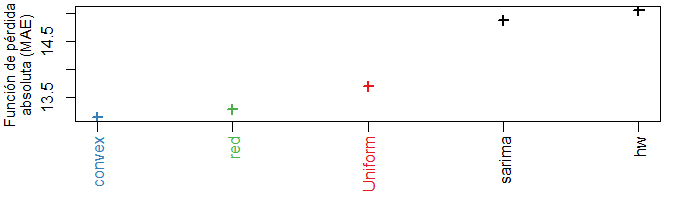
\includegraphics[scale = 0.7]{Images/Modelizacion/333.png}}
    \caption{Comparación del rendimiento entre modelos y combinaciones}
    \label{rendimiento}
\end{figure}

Vamos a hacer lo mismo solo que combinando linealmente las predicciones. Para ello pasaremos el argumento $\verb!model!$ como $\verb!linear!$. La comparativa del rendimiento se muestra en la Figura \ref{rendimiento_2}. Se puede apreciar como la combinación lineal es la que mejores resultados parece ofrecer, superando incluso a la convexa, sin embargo si estudiamos su ajuste en la Figura \ref{lin_conv} vemos que parece ajustarse muy bien en todo el conjunto de test menos en el pico correspondiente al mes de agosto. Aunque en este caso estamos obteniendo un MAE muy bajo la predicción no parece detectar este tipo de picos por lo que quizás no nos merecería la pena utilizarla.
\begin{figure}
    \centering
    \centerline{\includegraphics[scale = 0.7]{Images/Modelizacion/335.png}}
    \caption{Comparación del rendimiento entre modelos y combinaciones}
    \label{rendimiento_2}
\end{figure}

\begin{figure}
    \centering
    \centerline{\includegraphics[scale = 0.7]{Images/Modelizacion/336337.png}}
    \caption{Ajuste de las combinaciones convexa y lineal al \textit{test}}
    \label{lin_conv}
\end{figure}

Este tipo de combinaciones nos permiten tener en cuenta a la hora de predecir los aspectos de varios modelos, sin embargo por la naturaleza de la estimación están limitados a trabajar con conjuntos de datos completos. Una posible forma de implementar esto en línea sería iterando la estimación de las ponderaciones con todo el conjunto de datos más las nuevas observaciones que fuesen entrando pero para sistemas grandes resultaría muy costoso computacionalmente, además de que se podría incurrir a problemas de índole estadística.

\subsection{Combinaciones en línea}
El método $\verb!mixture()!$ nos permite definir lo que se conocen como \textit{aggregation rules}. Este tipo de técnicas actualizan las ponderaciones secuencialmente permitiendo así el entrenamiento en línea. Su sintaxis es la siguiente:
\begin{Verbatim}[fontsize=\footnotesize]
mixture(Y = NULL, experts = NULL, model = "MLpol", loss.type = "square",
        loss.gradient = TRUE, coefficients = "Uniform", parameters = list())
\end{Verbatim}

A través de $\verb!Y!$ introducimos las observaciones del \textit{test}, en $\verb!experts!$ las predicciones realizadas por los modelos y en $\verb!loss.type!$ la función de pérdida sobre la que trabajaremos. El tipo de \textit{aggregation rule} a usar se define a través de $\verb!model!$. Hay varias opciones, algunas de ellas ponderan exponencialmente las predicciones respecto al tiempo, otras aplican algunas técnicas de optimización más complejas, etc…  El argumento $\verb!loss.gradient!$ hace que se trabaje sobre el gradiente de la función de pérdida mientras que $\verb!coefficients!$ determina los valores iniciales de las ponderaciones, por defecto viene como $\verb!Uniform!$ para no dar así prioridad a unos modelos sobre otros. Algunas de estas \textit{aggregation rules} dependen de ciertos parámetros que pueden ser clave para obtener unos resultados óptimos, el argumento $\verb!parameters!$ se encarga de controlarlos. Si se deja por defecto estima los parámetros secuencialmente, en caso contrario se le debe introducir valores para los parámetros y él seleccionará aquellos que ofrezcan un mejor resultado.

Lo más común es pasar los argumentos $\verb!Y!$ y $\verb!experts!$ vacíos ($\verb!NULL!$) haciendo que el método solo defina la estructura de la \textit{aggregation rule} a utilizar. Para predecir se utiliza $\verb!predict()!$ de la librería $\verb!opera!$. Su sintaxis se muestra a continuación.
\begin{Verbatim}[fontsize=\footnotesize]
predict(object, newexperts = NULL, newY = NULL,
        type = c("model", "response", "weights", "all"), ...)
\end{Verbatim}

A través de $\verb!object!$ se introduce el objeto definido por $\verb!mixture()!$, en $\verb!newexperts!$ y $\verb!newY!$ se va introduciendo secuencialmente las predicciones de los modelos y sus respectivos valores en el \textit{test}. El argumento $\verb!type!$ indica al método la salida que debe ofrecer. Recomiendo dejar este último por defecto para obtener todo de una vez.

Vamos a implementar una \textit{aggregation rule} con ponderaciones exponenciales en el tiempo ($\verb!EWA!$). El parámetro $\verb!eta!$ controlará  la rapidez con la que aprenderá de los valores del \textit{test} y de las estimaciones de los modelos, en este caso vamos a dejar que el método los estime internamente. Seguiremos trabajando con la función de pérdida absoluta e iniciaremos los coeficientes uniformemente. Primero iniciaremos la \textit{aggregation rule}:
\begin{Verbatim}[fontsize=\footnotesize, numbers = left]
mix <- mixture(model = "EWA", loss.type = "absolute", coefficients = "Uniform")
\end{Verbatim}

Después para hacerlo más intuitivo vamos a ir iterando observación a observación del \textit{test}. El código se muestra a continuación:
\begin{Verbatim}[fontsize=\footnotesize, numbers = left]
model <- mix
for (i in 1:length(as.vector(acc.test))) {
  model <- predict(model, X[i,], as.vector(acc.test)[i])
}
\end{Verbatim}

En cada iteración las ponderaciones se irán ajustando de acuerdo a la discrepancia entre las predicciones de los distintos modelos y la correspondiente observación del \textit{test}. De esta forma la \textit{aggregation rule} aprenderá de los errores cometidos por las predicciones y dará más importancia a unos modelos u otros. En nuestro caso solo hemos realizado 12 iteraciones. Si hacemos $\verb!print()!$ sobre el $\verb!model!$ resultante obtenemos lo siguiente:
\begin{Verbatim}[fontsize=\footnotesize]
          Aggregation rule: EWA
          Loss function:  absolute loss
          Gradient trick:  TRUE
          Coefficients:
          red   sarima      hw
            1 1.31e-05 4.2e-11
\end{Verbatim}

En este caso vemos que las ponderaciones finales para estos tres modelos son de 1 para la red neuronal y de prácticamente 0 para el SARIMA y el suavizado Holt-Winters. La \textit{aggregation rule} ha decidido dar todo el peso de la predicción a la red. Esto significa que si quisiésemos predecir el mes de enero de 1976 tendríamos que ponderar las predicciones de los tres modelos de esta forma. Con el \textit{subsseting} $\verb!$weights!$ vemos la evolución de las ponderaciones durante el proceso de estimación. En nuestro caso tenemos lo siguiente:
\begin{Verbatim}[fontsize=\footnotesize]
                     red       sarima        hw
          [1,] 0.3333333 3.333333e-01 0.3333333
          [2,] 0.6190265 7.268057e-10 0.3809735
          [3,] 0.4593810 3.786922e-02 0.5027498
          [4,] 0.3251488 3.166993e-01 0.3581519
          [5,] 0.3325841 3.319613e-01 0.3354546
          [6,] 0.3333720 3.327050e-01 0.3339230
          [7,] 0.3333242 3.332837e-01 0.3333921
          [8,] 0.3333340 3.333242e-01 0.3333418
          [9,] 0.3333317 3.333336e-01 0.3333347
         [10,] 0.3333331 3.333335e-01 0.3333334
         [11,] 0.3333333 3.333334e-01 0.3333333
         [12,] 0.3333333 3.333333e-01 0.3333333
\end{Verbatim}

Vemos que comienza con ponderaciones uniformes pero ya en la segunda iteración distribuye el peso entre la red y el suavizado dejando al SARIMA sin voz en la predicción. En la tercera da más peso al suavizado que a la red y sigue dejando al SARIMA casi en cero. Tras esto las ponderaciones parecen evolucionar uniformemente. En la Figura \ref{mix} se puede observar el ajuste de las predicciones ponderadas. En este caso estamos obteniendo un MAE de 14.07949.
\begin{figure}
    \centering
    \centerline{\includegraphics[scale = 0.7]{Images/Modelizacion/337.png}}
    \caption{Ajuste de las predicciones de \PVerb{mix} con el \textit{test}}
    \label{mix}
\end{figure}

Si le pasamos el método $\verb!plot()!$ al objeto $\verb!model!$ obtenemos varios gráficos muy interesantes (la salida completa se muestra en el Anexo X). En la Figura \ref{entre_modelos}  se muestra la comparativa del rendimiento de la combinación con los modelos individuales. Podemos apreciar como el mejor MAE lo tiene la red neuronal seguida por la combinación uniforme de predicciones y por la aggregation rule.

Este tipo de combinaciones funcionan bien para modelos cuyas predicciones correlacionen poco, ya que esto significa que cada uno está recogiendo una parte del proceso que genera los datos, sin embargo a veces consigue afinar las predicciones entre modelos correlacionados. En nuestro caso la red neuronal producía unas predicciones muy suavizadas y el SARIMA y suavizado Holt-Winters parecían mostrar más picos. Combinando las tres obtenemos una predicción que consigue aunar estas cualidades, mostrando un comportamiento suave con algunos picos en variaciones de la serie significativas. Además, estudiando las ponderaciones, podemos ver qué modelos poseen un mayor poder predictivo pudiendo así orientar nuestro tiempo y recursos a mejorarlos.
\begin{figure}
    \centering
    \centerline{\includegraphics[scale = 0.7]{Images/Modelizacion/339.png}}
    \caption{{Comparación del rendimiento entre modelos, combinaciones y \PVerb{mix}}}
    \label{entre_modelos}
\end{figure}










\part{Conclusiones}
\lhead [\thepage]{V. Conclusiones}
\rhead [V. Conclusiones]{\thepage}

La elaboración de esta guía nos ha permitido obtener un conocimiento más profundo sobre el análisis de series temporales en $\textsf{R}$.

En ocasiones, la parte más laboriosa es la de la estructuración de los datos. Hay que tener cuidado a la hora de generar la fecha, pues $\textsf{R}$ no destaca en el tratamiento de este tipo de objetos. En este caso la clase $\verb!ts!$ acepta fechas sin necesidad de introducir objetos de clase $\verb!date!$, por lo que nos puede resultar útil cuando la serie está estructurada regularmente, sin embargo las clases $\verb!zoo!$ y $\verb!xts!$ se adaptan mejor a tiempos irregulares. Los métodos orientados al tratamiento de $\verb!NAs!$ incluidos en la librería $\verb!zoo!$ funcionan muy bien y son realmente útiles. Además si queremos hacer algún tratamiento sencillo de los datos podemos hacerlo, con métodos como $\verb!rollmean()!$ y $\verb!rollapply()!$. La librería $\verb!xts!$ implementa una conversión entre clases más sencilla por lo que quizás convendría inclinarse más hacia ella que hacia $\verb!zoo!$. Si se necesita hacer algún tratamiento de los datos conviene utilizar $\verb!zoo!$ o $\verb!xts!$ y en el momento en el que tengamos la serie lista la convertimos a la clase $\verb!ts!$ ya que, pese a su sencillez, es la que más se usa y la que, por tanto, menos problemas da cuando se utiliza con métodos de librerías externas.

Uno de los puntos fuertes de la librería $\verb!forecast!$ es su variedad ya que incluye una gran cantidad de métodos encargados de implementar distintos modelos, la mayor parte de ellos orientados a la predicción. Esta variedad nos permite diseñar una búsqueda del modelo óptimo basada en la complejidad, es decir, podemos comenzar con modelos sencillos e ir ascendiendo en complejidad hasta encontrar uno que sin ser excesivamente complejo nos ofrezca los resultados que buscamos. Además nos aporta métodos orientados al preprocesado de la serie, pudiendo diferenciar, descomponer, introducir rezagos, aplicar test de raíz unitaria o estudiar la estacionalidad sin necesidad de recurrir a otra librería. Una vez ajustado un modelo es sencillo predecir con él y comparar los resultados con el conjunto de \textit{test}, pudiéndose obtener una gran cantidad de medidas de precisión. También incluye métodos muy útiles para estudiar los residuos y comprobar si efectivamente son ruido blanco.

La librería $\verb!TSeries!$ no es tan completa como $\verb!forecast!$ pero contiene métodos muy útiles. Implementa multitud de test estadísticos, los cuales pueden sernos de gran utilidad para conocer bien nuestra serie, a fin de ajustarla un modelo u otro. Además implementa también técnicas de remuestreo, algo difícil de encontrar en este tipo de librerías. Al no tener métodos orientados al preprocesado es necesario recurrir a otras librerías. Únicamente implementa modelos ARMA, por lo que este preprocesado es indispensable. Una vez ajustado el modelo no nos da la opción de predecir con él, por lo que necesitaríamos escribir una función que se encargase de esto, algo que puede llegar a ser realmente laborioso.

La librería $\verb!FitARMA!$ es similar a $\verb!TSeries!$ solo que esta está orientada únicamente a ajustar modelos ARIMA. Se caracteriza por el algoritmo que utiliza para la estimación. En teoría este algoritmo hace que el método ajuste el modelo con un menor coste computacional en comparación a otras librerias, sin embargo hemos visto que los que mejores tiempos se obtienen con los métodos de $\verb!forecast!$ y  $\verb!TSeries!$.

La librería $\verb!opera!$ nos permite mejorar las predicciones mediante la combinación de varios modelos. Nos permite realizar estas combinaciones teniendo o no en  cuenta el tiempo, además algunos métodos ofrecen gráficos muy útiles que nos ayudan a visualizar los resultados. Es una librería algo más complicada de utilizar que las anteriores pero nos puede dar muy buenos resultados.

El ciclo de vida de los datos temporales en $\textsf{R}$ desarrollado en este trabajo se puede resumir en las siguientes etapas:

\begin{itemize*}
  \item[$\bullet$] \textbf{Estructuración}: Apoyarnos en las librerías $\verb!zoo!$ y $\verb!xts!$ para dar forma a los datos si es necesario. Convertir el objeto final en uno de clase $\verb!ts!$.
  \item[$\bullet$] \textbf{Preprocesado}: Utilizar la librería $\verb!forecast!$. Podemos apoyarnos en métodos de la librería $\verb!TSeries!$.
  \item[$\bullet$] \textbf{Modelización}: Con $\verb!forecast!$ debería ser suficiente. Podemos apoyarnos en $\verb!TSeries!$ y $\verb!FitARMA!$, aunque no suele ser necesario.
  \item[$\bullet$] \textbf{Validación}: $\verb!Forecast!$ posee muchos métodos para evaluar los modelos ajustados.
  \item[$\bullet$] \textbf{Predicción}: Las predicciones iniciales las hacemos con $\verb!forecast!$. Si hemos ajustado más de un modelo podemos mejorar los resultados con $\verb!opera!$.
\end{itemize*}







\renewcommand{\refname}{Bibliografía}

\bibliographystyle{apacite}
\bibliography{referencias-TFG}
\lhead [\thepage]{Bibliografía}
\rhead [Bibliografía]{\thepage}

\end{document}
